%%%%%%%%%%%%%%%%%%%%%%%%%%%%%%%%%%%%%%%%%%%%%%%%%%%%%%%%%%%%%%%%%
\section{Phân tích yêu cầu hệ thống}
Hệ thống có thể được sử dụng bởi số lượng lớn người dùng. Mỗi ngừời dùng/quản lý sẽ có một tài khoản riêng cho mình. Mỗi tài khoản sẽ có một số lĩnh vực được cho phép sử dụng các chức năng khác nhau nằm trong quyền hạn của mình. Hệ thống website du lịch có thể được tóm gọn trong các chức năng như sau: 
\subsection{Quản trị viên}
Quản trị viên có toàn quyền sử dụng bất cứ chức năng nào của hệ thống như quản lý người dùng:
\begin{itemize}
    \item Hiển thị danh sách toàn bộ người dùng, bài viết, thông tin kế hoạch chuyến đi. 
    \item Quản lý thông tin người dùng: thông tin bao gồm các thông tin cá nhân và một số thông tin của người thân. Hệ thống cho phép chỉnh sửa và cập nhật khi thông tin có thay đổi.
    \item Hiển thị, thêm, xoá, sửa vai trò và quyền của người dùng.
    \item Hiện thị, thêm, xoá, sửa các bảng danh mục.
    \item Quản lý thông tin bài review.
    \item Quản lý thông tin chuyến đi.
    \item Quản lý thông tin cộng tác viên.
    \item Quản lý thông tin bình luận, đánh giá của bài review và chuyến đi.
\end{itemize}
\subsection{Cộng Tác Viên}
\begin{itemize}
    \item Cấu hình giá.
    \item Hiện thị, thêm, xoá, sửa sự kiện.
    \item Nếu không có quyền tạo sự kiện thì sự kiện được tự động tạo bản nháp và chờ người có quyền duyệt.
    
\end{itemize}
\subsection{Người dùng}
\begin{itemize}
    \item Quản lý thông tin cá nhân.
    \item Quản lý bài review.
    \item Quản lý thông tin chuyến đi.
    \item Quản lý thông tin bình luận của mình trong bài review.
        \subitem 
\end{itemize}
\subsection{Gửi thông báo bằng email}
Hệ thống gửi thông báo qua email khi có những hành động liên quan đến các sự kiện và thông tin chuyến đi:
\begin{itemize}
    \item Thông báo bài viết đã được phê duyệt.
    \item Khi một người dùng đăng ký tham chuyến đi. 
    \item Thông báo khi kế hoạch chuyến đi đã đủ người tham gia.
\end{itemize}
\section{Tổng quát kiến trúc hệ thống}
\indent 
    Hệ thống được xây dựng theo mô hình MVC kết hợp với REST API (RESTful). Ngoài ra để xử lý các tác vụ real time, nhóm sử dụng lớp Socket.io ở giữa tầng View và Controller.
Vận dụng kiến trúc REST API trong hệ thống:
Các API trong hệ thống Website du lịch Goz được thiết kế theo các nguyên tắc chung, nhất quán giữa các module.
\begin{itemize}
    \item API được đặt tên theo quy định chung, phù hợp với công dụng, quyền của API, thống nhất giữa các module.
    \begin{itemize}
        \item \textit{``/api/event/page/:pageNumber/:pageSize''}: API lấy tất cả dữ liệu của một bảng sự kiện. Ta có thể thấy các API có cấu trúc thống nhất với nhau với các bảng khác.
        \item \textit{``/api/draft-event/item/:eventId''}: API lấy dữ liệu của bảng sự kiện theo ID.
    \end{itemize}
    \item Sử dụng các phương thức HTTP (GET, POST, PUT, DELETE) để truy cập và xử lý dữ liệu.
    \begin{itemize}
        \item  \textit{GET /api/event/page/:pageNumber/:pageSize}: cách dùng API để lấy dữ liệu.
        \item  \textit{POST /api/event/default}: cách dùng API để thêm dữ liệu.
        \item  \textit{PUT /api/event/swap}: cách dùng API để sửa đổi dữ liệu.
        \item  \textit{DELETE /api/draft-event}: cách dùng API để xoá dữ liệu.
    \end{itemize}
    \item Dữ liệu được server trả về theo định dạng JSON.
    \item Server trả về các HTTP code phù hợp.
    \begin{itemize}
        \item  400 Invalid parameter: Trả về lỗi này khi client gửi yêu cầu sai cú pháp.
        \item  403 Can not access data: Trả về lỗi này khi client không có quyền truy cập dữ liệu.
        \item  404 Not found: Trả về lỗi này khi server không tìm thấy dữ liệu client yêu cầu.
    \end{itemize}
\end{itemize}

Nhận thấy mô hình MVC có nhiều ưu điểm và phù hợp với hệ thống (trình bày ở mục 2.1 Mô hình Model-View-Controller) nên nhóm đã sử dụng mô hình này trong thiết kế kiến trúc hệ thống.\\

Vận dụng mô hình MVC trong hệ thống Website du lịch Goz:
\begin{center}
  \captionsetup{type=figure}
  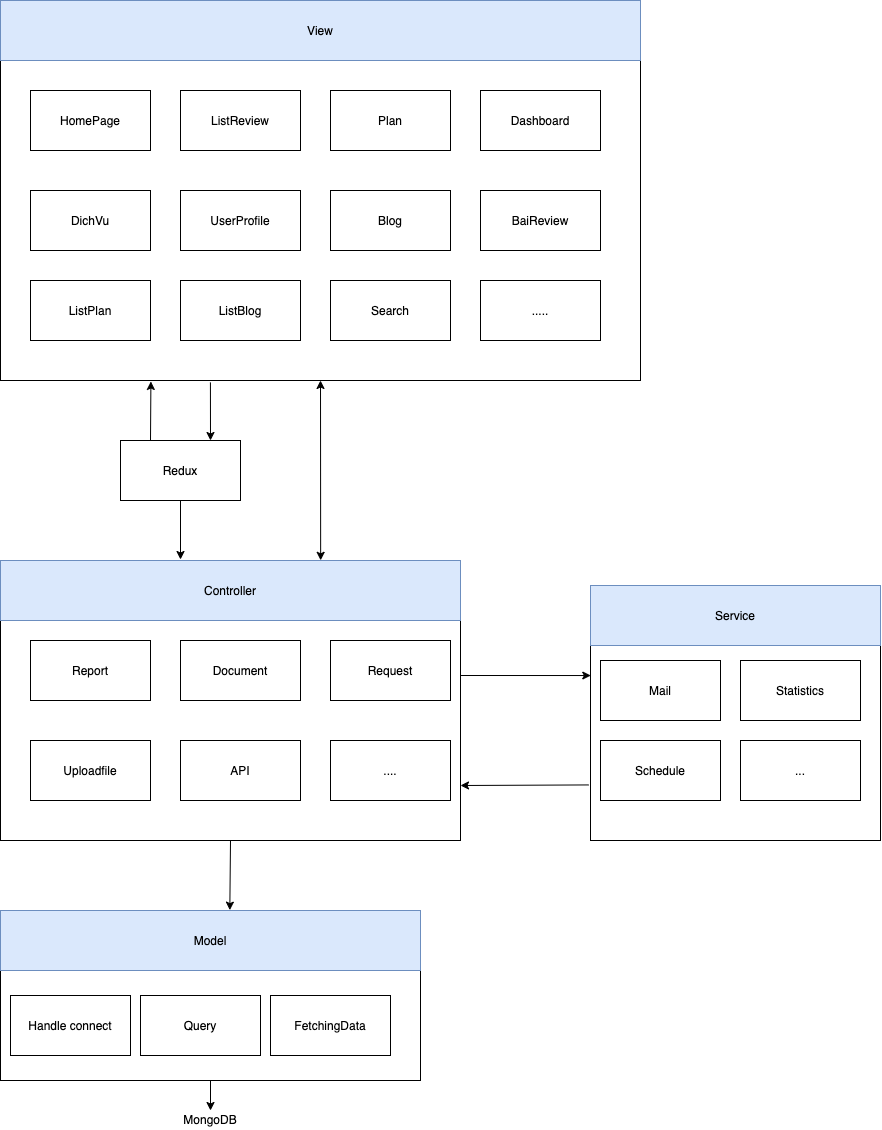
\includegraphics[width=15cm]{image/MVC11.png}
  \captionof{figure}{Kiến trúc tổng thể của hệ thống}
\end{center}

\section{Thiết kế đối tượng người dùng}
\subsection{Danh sách đối tượng người dùng}
Dựa vào những yêu cầu thực tế của hệ thống và những khảo sát thực tế đối với các cá nhân có nhu cầu sử dụng, xây dựng hệ thống Website du lịch Goz. Nhóm đưa ra các vai trò, người dùng chính trong hệ thống như sau:
\begin{table}[H]
    \centering
	\begin{tabular}{|p{1cm}|p{4cm}|p{10cm}|}
    \hline
    \textbf{STT}&\textbf{Người dùng}&\textbf{Đặc tả}\\
    \hline
    1&Khách&Là những người dùng chưa đăng nhập, bao gồm tất cả các đối tượng truy cập vào website như học sinh, sinh viên, phụ huynh, đơn vị, doanh nghiệp,...
    
    Khách có chức năng xem thông tin, tin tức, sự kiện, bài review của website, gửi email liên hệ,đăng kí và đăng nhập.\\
    \hline
	2&Người dùng ( thành viên đã đăng kí )& Người sử dụng có thể sử dụng tất cả các chức năng của trang web như tạo lịch trình chuyến đi cũng như đăng bài review, chia sẻ thông tin chuyến đi của mình với bạn bè. \\
	\hline
    3&Quản lí trang web& Người quản lí thông tin tất cả các tài khoản người dùng, duyệt bài review chuyến đi.\\
   
	\hline
\end{tabular}
\caption{Danh sách đối tượng người dùng của hệ thống}
\end{table}
\begin{center}
  \captionsetup{type=figure}
  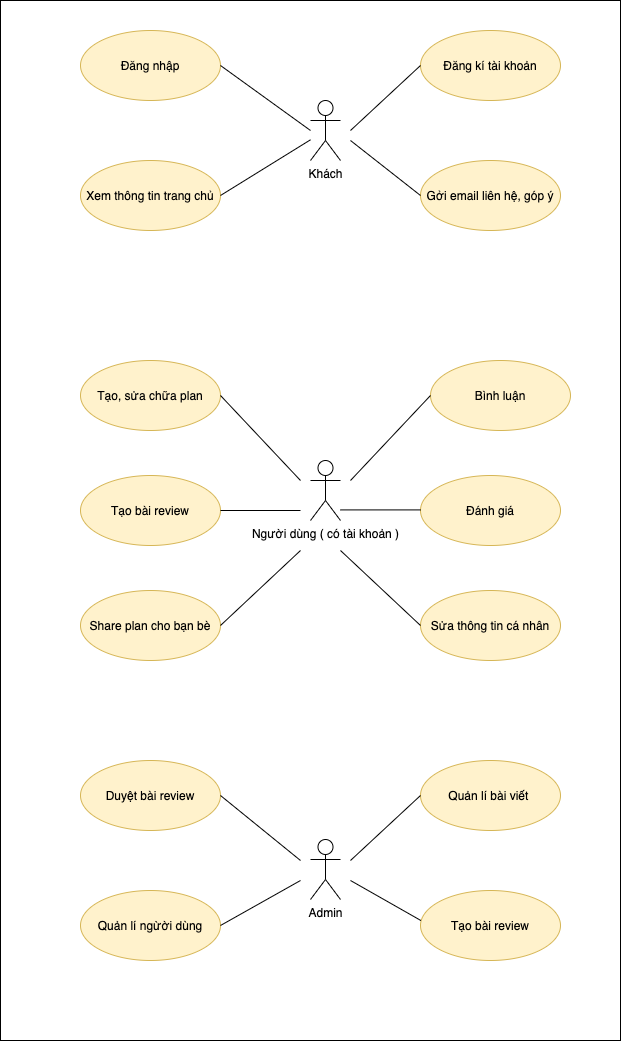
\includegraphics[width=14cm]{document/image/List3ND.png}
  \captionof{figure}{Lược đồ Usecase các đối tượng của hệ thống }
\end{center}
% \subsection{Đối tượng: Quản trị hệ thống}
% \textbf{Lược đồ Usecase đối tượng quản trị hệ thống}
% \begin{center}
%   \captionsetup{type=figure}
%   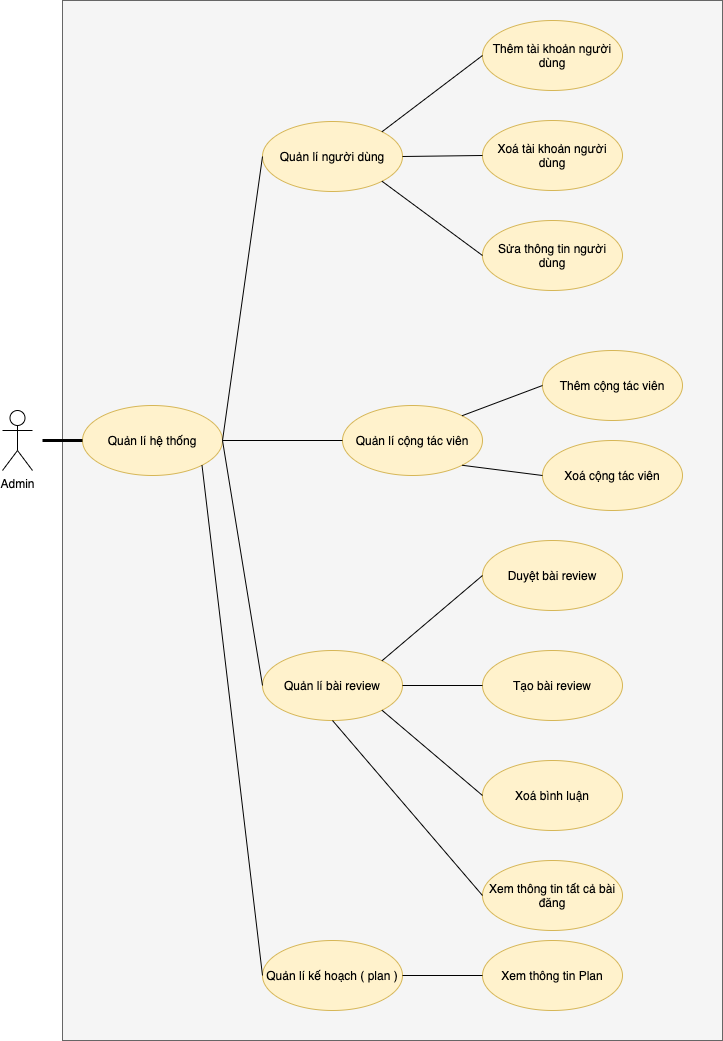
\includegraphics[width=13cm]{document/image/useCaseAdmin.png}
%   \captionof{figure}{Lược đồ usecase của đối tượng quản trị hệ thống}
% \end{center}

% \indent Đối với đối tượng là quản trị hệ thống, sau khi xác thực thành công sẽ có những nhóm chức năng: quản lí người dùng, quản lí cộng tác viên, quản lí bài review và quản lí kế hoạch. Với mỗi nhóm chức năng sẽ có những chức năng tương ứng sau:

% \begin{itemize}
%     \item Nhóm quản lý tài khoản người dùng & tài khoản cộng tác viên bao gồm các chức năng:
%         \subitem - Xem thông tin các tài khoản.
%         \subitem - Tạo mới tài khoản.
%         \subitem - Xoá tài khoản người dùng.
%         \subitem - Chỉnh sửa thông tin tài khoản.
%         \subitem - Thêm và xoá vai trò cho tài khoản.
    
%     \item Nhóm quản lý bài review:
%         \subitem - Phê duyệt bài review người dùng đăng.
%         \subitem - Xem danh sách tất cả các bài viết.
%         \subitem - Tạo mới và xoá bài viết.
%         \subitem - Quản lí bình luận người dùng.
%         \subitem - Duyệt bài viết người dùng.
%     \item Chắc năng quản lí kế hoạch chỉ cho phép quản lí hệ thống chỉ có thể xem thông tin các kế hoạch mà người dùng đã tạo mà không thể can thiệp quá sâu.
%     \item Ngoài ra nhóm quản lí có thể cấu hình giao diện trang chủ, cấu hình thông tin trang web, cấu hình email cho hệ thống.
%         \subitem - Cấu hình giao diện trang chủ: Tùy chỉnh các thành phần giao diện, lựa chọn các thành phần giao diện sẽ xuất hiện ở trang chủ.
%         \subitem - Cấu hình thông tin trang web: Cấu hình các thông tin chung cho hệ thống.
%         \subitem - Cấu hình email hệ thống: Tủy chỉnh các mẫu email tự động của hệ thống.
% \end{itemize}
\subsection{Đối tượng: Khách}
\textbf{Lược đồ Usecase đối tượng khách}
\begin{center}
  \captionsetup{type=figure}
  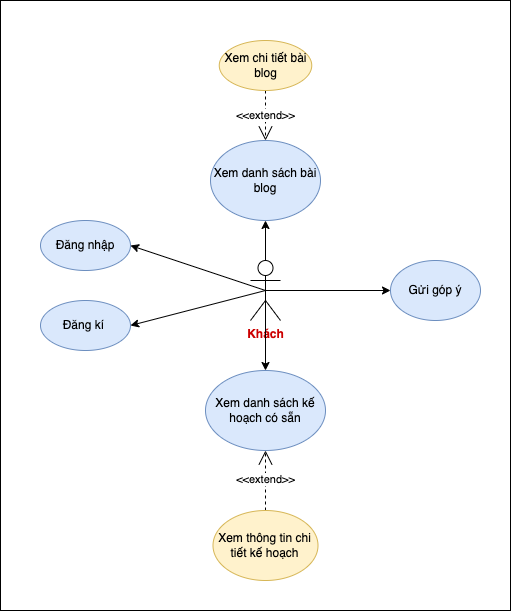
\includegraphics[width=14cm]{document/image/usecaseKhach2.png}
  \captionof{figure}{Lược đồ Usecase của đối tượng khách}
\end{center}

Khách là những người dùng chưa đăng nhập, bao gồm tất cả các đối tượng như học sinh,  sinh viên, phụ huynh, đơn vị, doanh nghiệp là đối tác của Website,...
 
 Đối tượng khách có thể truy cập trang chủ để xem các thông tin chung, thông tin liên hệ, xem các tin tức và sự kiện, bài review, thông tin chuyến đi. Khi có nhu cầu liên hệ với Goz, khách có thể vào mục liên hệ để gửi email để liên lạc hoạt gọi hotline để được hỗ trợ trực tiếp.
 
\clearpage
\subsection{Đối tượng: Người dùng ( đã có tài khoản )}
\textbf{Lược đồ Usecase đối tượng người dùng}
\begin{center}
  \captionsetup{type=figure}
  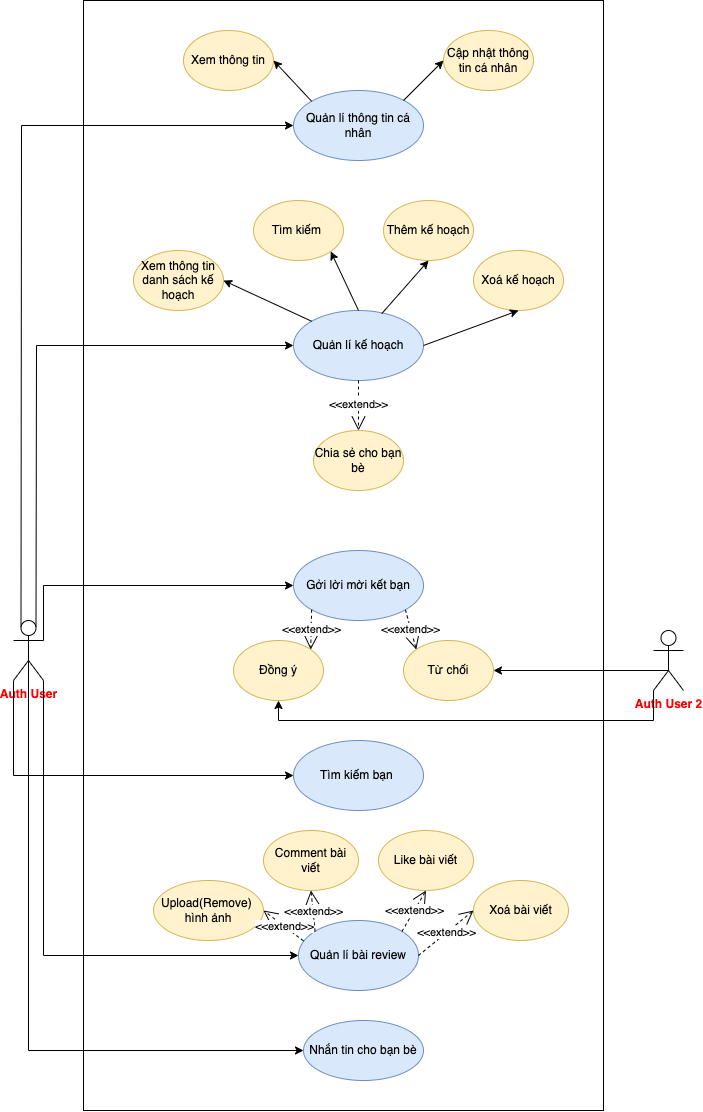
\includegraphics[width=14cm]{document/image/usecaseAuthUser.drawio.png}
  \captionof{figure}{Lược đồ Usecase đối tượng người dùng}
\end{center}

Đối với người dùng đã có tài khoản đăng nhập, sau khi đăng nhập sẽ  có các chức năng như sau: 
\begin{itemize}
    \item Quản lí thông tin cá nhân:
        \subitem - Xem và sửa các thông tin cá nhân.
    \item Quản lí kế hoạch:
        \subitem - Xem và sửa các thông tin kế hoạch chuyến đi.
        \subitem - Tạo kế hoạch mới.
        \subitem - Xoá kế hoạch.
        \subitem - Chia sẻ kế hoạch với bạn bè.
        
    \item Quản lí bài review:
        \subitem - Tạo bài review mới.
        \subitem - Bình luận bài review.
        \subitem - Thích bài review
        \subitem - Đánh giá.
    \item Tương tác với người dùng khác: 
    \subitem - Tìm kiếm bạn bè.
    \subitem - Gởi lời mời kết bạn.
    \subitem - Đồng ý hoặc từ chối lời mời kết bạn từ người khác.
    \subitem - Nhắn tin cho bạn bè.
     
    
\end{itemize}

\clearpage
% \subsection{Đối tượng: Quản lý ( admin )}
% \textbf{Lược đồ Usecase đối tượng quản lý}
% \begin{center}
%   \captionsetup{type=figure}
%   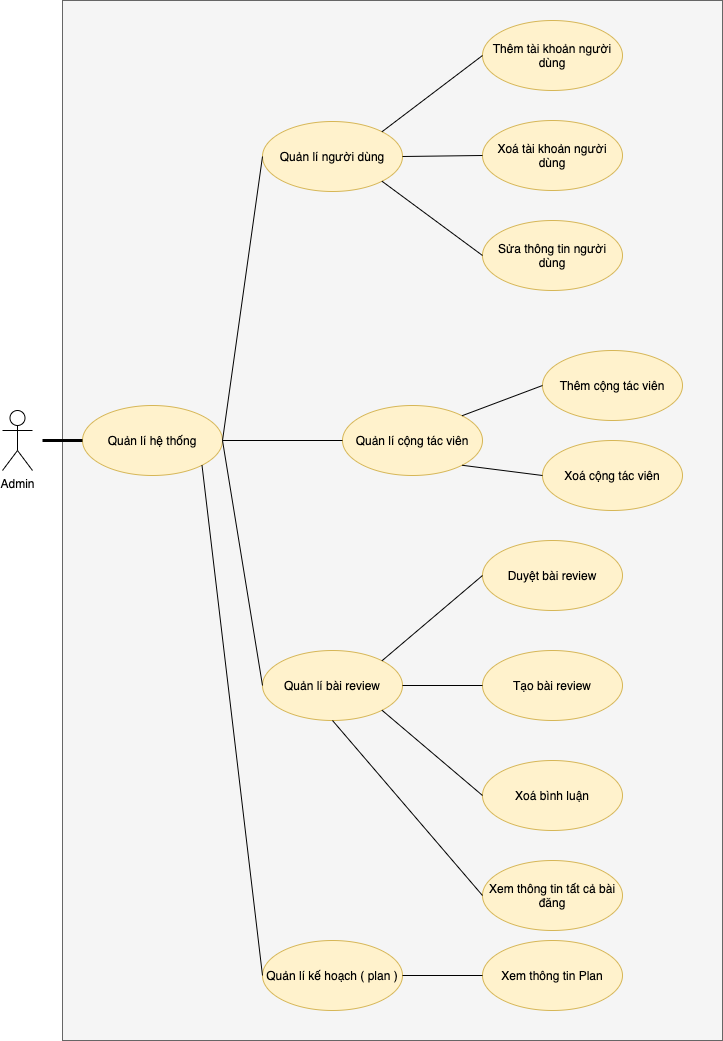
\includegraphics[width=15cm]{document/image/useCaseAdmin.png}
%   \captionof{figure}{Lược đồ Usecase đối tượng quản lý ( admin )}
% \end{center}

% Sau khi đăng nhập vào hệ thống, người dùng là quản lý sẽ có các nhóm chức năng sau: quản lý, tạo và đăng bài review các địa điểm du lịch mới. Phê duyệt bài review do người dùng đăng.

% Chức năng quản lý bài review bao gồm xem danh sách toàn bộ bài review, tạo mới, sửa đổi và xoá bài review.

% Chức năng quản lí cộng tác viên bao gồm thêm ( xoá ) tài khoản cộng tác viên như chủ khách sạn, homestay, nhà hàng, ... .

% Chức năng quản lí kế hoạch ( plan ) chỉ có thể xem thông tin kế hoạch mà người dùng đã tạo.

% \clearpage

\section{Thiết kế cơ sở dữ liệu cho hệ thống}
\subsection{Lược đồ ERD}

Chi tiết xem ở tài liệu đính kèm.

\subsection{Lược đồ cơ sở dữ liệu}
\begin{center}
  \captionsetup{type=figure}
g  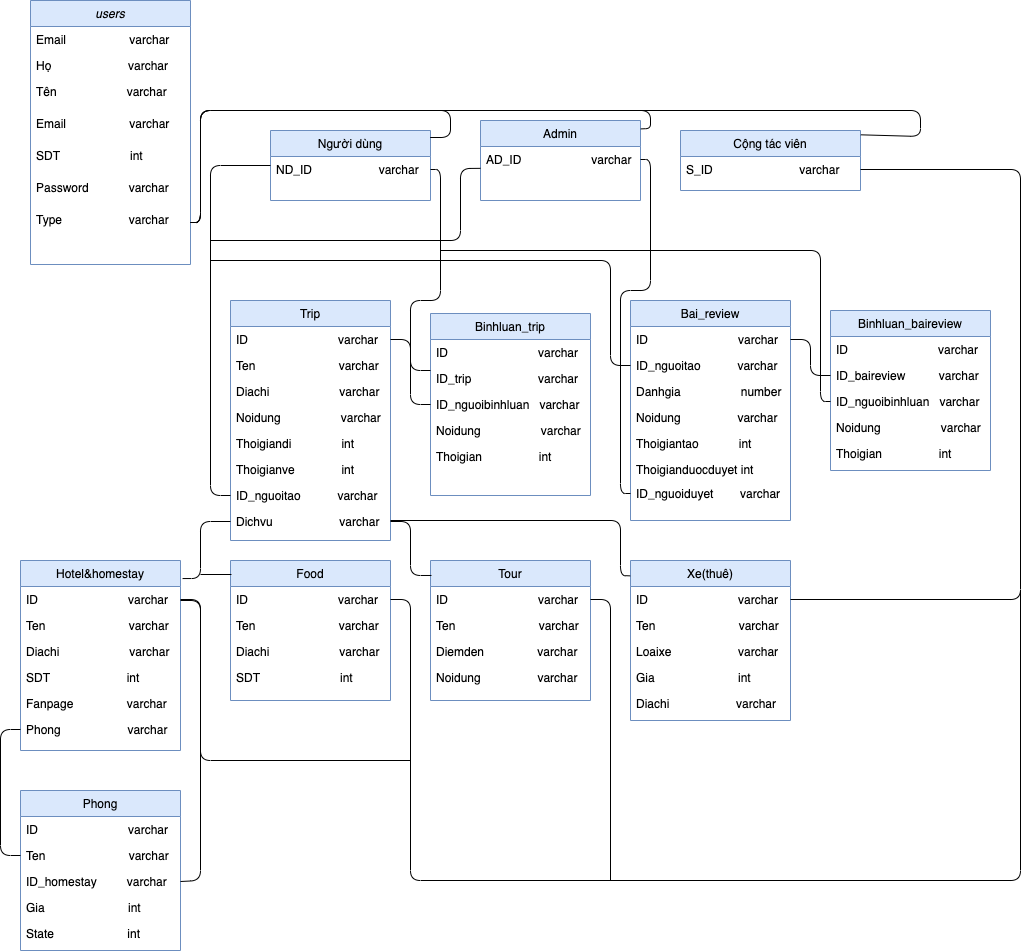
\includegraphics[width=\linewidth]{image/classDiagram.png}
  \captionof{figure}{Thiết kế cơ sở dữ liệu của hệ thống}
\end{center}
\section{Chức năng từng đối tượng trong hệ thống}
Từ việc thiết kế Usecase ở chương 4, nhóm nghiên cứu tiến hành thực hiện từng chức năng tương ứng với mỗi đối tượng. Cụ thể từng chức năng quan trọng như sau:

\subsection{Chức năng đăng kí tài khoản cá nhân.}\\
 Đặc tả usecase đăng ký tài khoản cá nhân:  

\begin{table}[H]
    \centering
	\begin{tabular}{|p{5cm}|p{10cm}|}
    % \hline
    % \textbf{Người dùng}&\textbf{Đặc tả}\\
    \hline
    Usecase Name&Đăng ký tài khoản cá nhân\\
    \hline
    Usecase Description&Người dùng muốn đăng kí tài khoản cá nhân\\
    \hline
    Post Condition&Hiển thị thông báo thành công và chuyển đến trang đăng nhập\\
    \hline
    Basic Flow& 1. Người dùng nhấn vào nút "Đăng ký" ở thanh sidebar.
    
    2. Chuyển đến trang đăng ký.
    
    3. Nhập họ tên.
    
    4. Nhập email.
    
    5. Nhập mật khẩu.
    
    6. Nhập lại mật khẩu.
    
    7. Nhập số điện thoại.
    
    8. Nhập ngày tháng năm sinh.
    
    9. Chọn giới tính.
    
    10. Nhập địa chỉ.
    
    11. Nhấn nút đăng ký.\\
    \hline Business Rules&- Email là duy nhất.
    
    - Số điện thoại đúng chuẩn và duy nhất.\\
   
   
	\hline
\end{tabular}
\caption{Usecase đăng ký tài khoản }
\end{table}

\begin{center}
    \captionsetup{type=figure}
    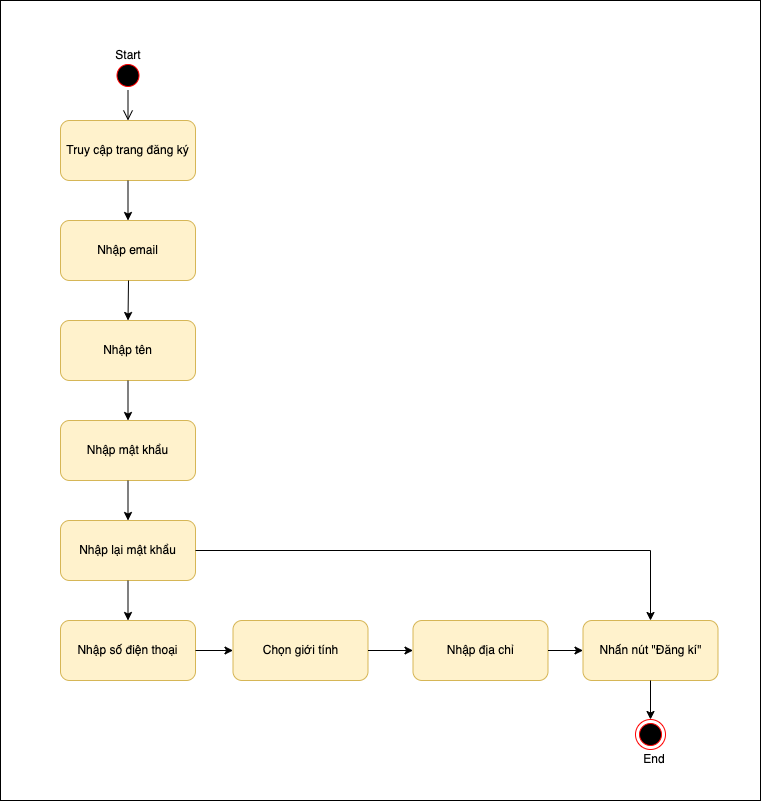
\includegraphics[width=12cm]{document/image/activityDK.drawio.png}
    \captionof{figure}{Lược đồ Activity đăng kí }
\end{center}

\subsection{Chức năng Lên kế hoạch và tạo chi tiết thông tin chuyến đi}
 Đặc tả usecase tạo kế hoạch:  
 \begin{table}[H]
    \centering
	\begin{tabular}{|p{5cm}|p{10cm}|}
    % \hline
    % \textbf{Người dùng}&\textbf{Đặc tả}\\
    \hline
    Usecase Name&Tạo kế hoạch chi tiết cho chuyến đi\\
    \hline
    Usecase Description&Người dùng muốn tạo kế hoạch chi tiết cho chuyến đi\\
    \hline
    Post Condition&Hiển thị thông báo thành công \\
    \hline
    Basic Flow& 1. Người dùng nhấn vào nút "Create Plan" ở thanh sidabar
    
    2. Chuyển đến trang tạo kế hoạch.
    
    3. Nhập ngày đi.
    
    4. Nhập ngày về
    
    5. Nhập địa điểm đến
    
    6. Nhấn nút "Create".
    
    7. Chuyển đến giao diện tất cả kế hoạch tính theo số ngày đi.
    
    8. Chọn kế hoạch muốn thêm hoạt động.
    
    9. Chuyển đến giao diện thêm hoạt động chi tiết cho chuyến đi.
    
    10. Nhập thời gian
    
    11. Chọn thể loại hoạt động.
    
    12. Chọn địa điểm cho hoạt động đó.
    
    13. Nhấn nút "Add"\\
    \hline Business Rules&- \\
   
   
	\hline
\end{tabular}
\caption{Usecase tạo kế hoạch }
\end{table}
 \begin{center}
  \captionsetup{type=figure}
  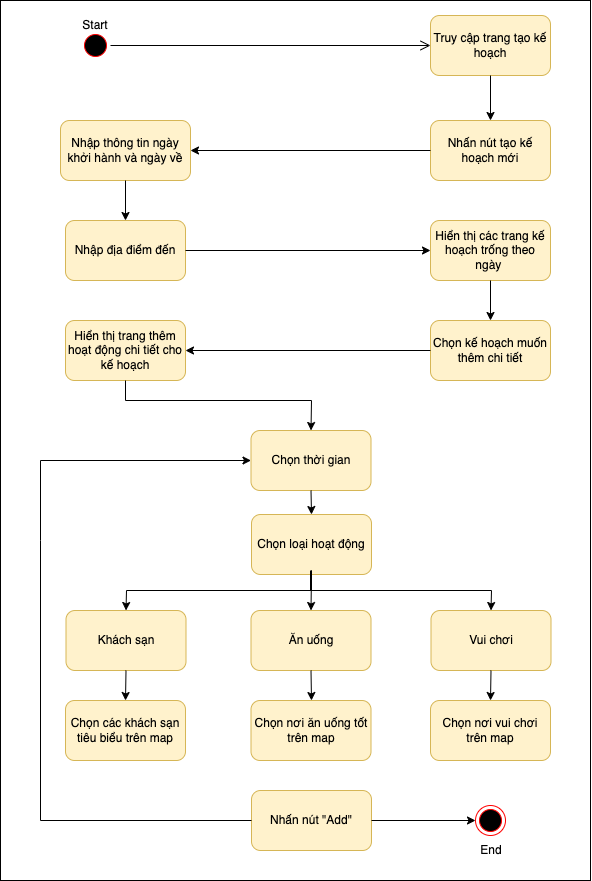
\includegraphics[width=12cm]{document/image/usecasePlan.drawio.png}
  \captionof{figure}{Lược đồ Activity tạo thông tin kế hoạch cho chuyến đi}
\end{center}

\subsection{Chức năng tạo vài blog về địa điểm vừa đi}

Đặc tả usecase tạo bài blog: 
\begin{table}[H]
    \centering
	\begin{tabular}{|p{5cm}|p{10cm}|}
    % \hline
    % \textbf{Người dùng}&\textbf{Đặc tả}\\
    \hline
    Usecase Name&Tạo bài blog\\
    \hline
    Usecase Description&Người dùng muốn tạo bài blog\\
    \hline
    Post Condition&Hiển thị thông báo thành công \\
    \hline
    Basic Flow& 1. Người dùng nhấn vào nút "Create Blog" ở thanh sidebar
    
    2. Chuyển đến trang tạo blog.
    
    3. Nhập địa điểm đã đi
    
    4. Upload hình ảnh
    
    5. Nhập trải nghiệm.
    
    6. Nhấn nút "Create".
    
    7. Thông báo thành công.\\
    

    \hline Business Rules& \\
   
   
	\hline
\end{tabular}
\caption{Usecase tạo bài blog }
\end{table}
 \begin{center}
  \captionsetup{type=figure}
  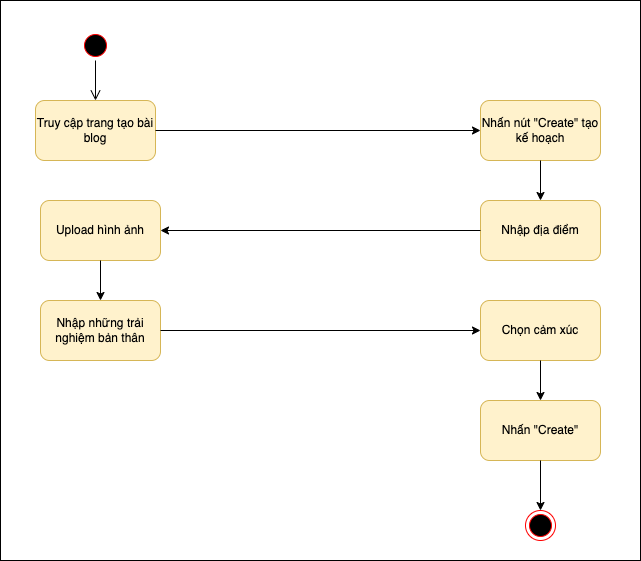
\includegraphics[width=12cm]{document/image/usecaseBlog.drawio.png}
  \captionof{figure}{Lược đồ Activity tạo bài blog}
\end{center}

\subsection{Chức năng kết bạn}
Đặc tả usecase kết bạn: 
\begin{table}[H]
    \centering
	\begin{tabular}{|p{5cm}|p{10cm}|}
    
    \hline
    Usecase Name&Kết bạn\\
    \hline
    Usecase Description&Người dùng muốn kết bạn với người dùng khác\\
    \hline
    Post Condition&Hiển thị thông báo gởi lời mời kết bạn thành công \\
    \hline
    Basic Flow& 1. Người dùng nhấn vào biểu tượng kết bạn hoặc nhấn vào ô "Search" để tìm người mình muốn kết bạn.
    
    2. Nhập tên người dùng muốn kết bạn.
    
    3. Nhấn "Add"
    
    4. Hiển thị thông bảo thành công\\
    

    \hline Business Rules& \\
   
   
	\hline
\end{tabular}
\caption{Usecase kết bạn}
\end{table}
 \begin{center}
  \captionsetup{type=figure}
  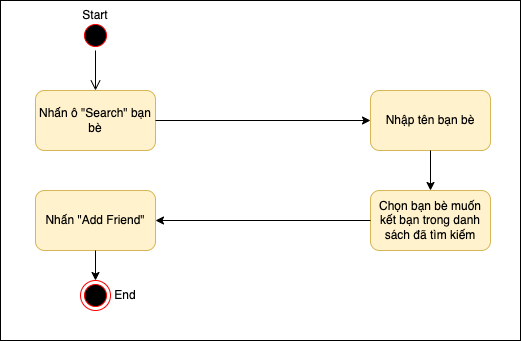
\includegraphics[width=12cm]{document/image/KetBan.drawio.png}
  \captionof{figure}{Lược đồ Activity kết bạn}
\end{center}

\subsection{Chức năng đồng ý và từ chối lời mời kết bạn}
Đặc tả usecase đồng ý và từ chối lời mời kết bạn: 
\begin{table}[H]
    \centering
	\begin{tabular}{|p{5cm}|p{10cm}|}
    
    \hline
    Usecase Name&Đồng ý hoặc từ chối lời mời kết bạn\\
    \hline
    Usecase Description&Người dùng muốn phản hồi lời mời kết bạn\\
    \hline
    Post Condition&Hiển thị thông báo chấp nhận ( từ chối ) lời mời thành công \\
    \hline
    Basic Flow& 1. Người dùng nhấn vào biểu tượng bạn bè trên thanh sidebar
    2. Hiển thị danh sách người dùng đã gởi lời mời kết bạn.
    
    3. Nhấn "Accecpt" để đồng ý hoặc "Decline" để từ chối.
    
    4. Hiển thị thông bảo thành công\\
    

    \hline Business Rules& \\
   
   
	\hline
\end{tabular}
\caption{Usecase đồng ý hoặc từ chối lời mời kết bạn}
\end{table}
 \begin{center}
  \captionsetup{type=figure}
  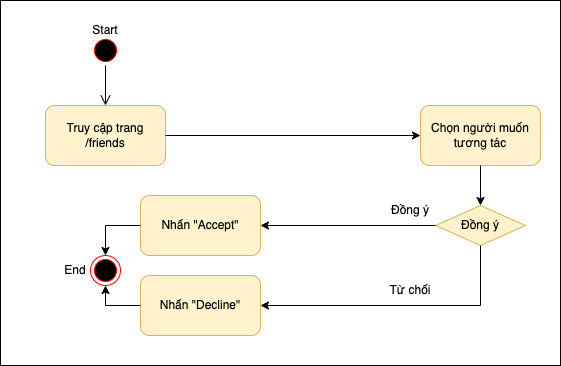
\includegraphics[width=12cm]{document/image/acKetban.drawio.png}
  \captionof{figure}{Lược đồ Activity đồng ý hoặc từ chối lời mời kết bạn}
\end{center}

\subsection{Chức năng Unfriend bạn}
Đặc tả usecase unfriend bạn: 
\begin{table}[H]
    \centering
	\begin{tabular}{|p{5cm}|p{10cm}|}
    
    \hline
    Usecase Name&Unfriend bạn\\
    \hline
    Usecase Description&Người dùng muốn xoá quan hệ bạn bè\\
    \hline
    Post Condition&Hiển thị thông báo xoá bạn bè thành công. \\
    \hline
    Basic Flow& 1. Người dùng nhấn vào ô "Search" để tìm bạn bè muốn unfriend.
    2. Hiển thị danh sách người dùng có tên vừa tìm kiếm.
    
    3. Chọn bạn bè muốn huỷ quan hệ bạn bè.
    
    4. Nhấn "Unfriend".
    
    5. Hiển thi thông báo thành công.\\
    

    \hline Business Rules& \\
   
   
	\hline
\end{tabular}
\caption{Usecase huỷ quan hệ bạn bè}
\end{table}
 \begin{center}
  \captionsetup{type=figure}
  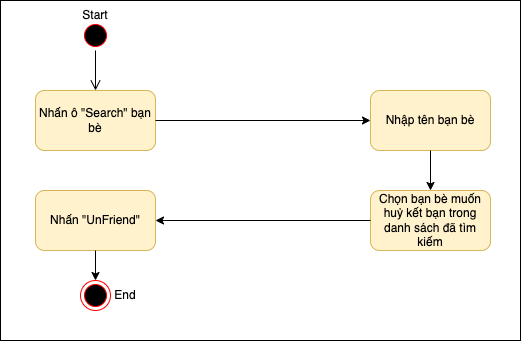
\includegraphics[width=12cm]{document/image/Unfriend.png}
  \captionof{figure}{Lược đồ Activity huỷ kết bạn}
\end{center}

\subsection{Chức năng nhắn tin với bạn bè}
Đặc tả usecase nhắn tin với bạn: 
\begin{table}[H]
    \centering
	\begin{tabular}{|p{5cm}|p{10cm}|}
    
    \hline
    Usecase Name&Nhắn tin với bạn bè\\
    \hline
    Usecase Description&Người dùng muốn nhắn tin với bạn bè\\
    \hline
    Post Condition&Hiển thị thông báo gởi tin nhắn thành công \\
    \hline
    Basic Flow& 1. Người dùng nhấn vào biểu tượng "Chat" trên thanh sidebar
    2. Hiển thị danh sách bạn bè.
    
    3. Chọn bạn bè muốn nhắn tin.
    
    4. Nhập thông tin cuộc hội thoại.
    
    5. Nhấn "Gửi"
    
    5. Hiển thi thông báo gửi tin nhắn thành công.\\
    

    \hline Business Rules& \\
   
   
	\hline
\end{tabular}
\caption{Usecase nhắn tin}
\end{table}
 \begin{center}
  \captionsetup{type=figure}
  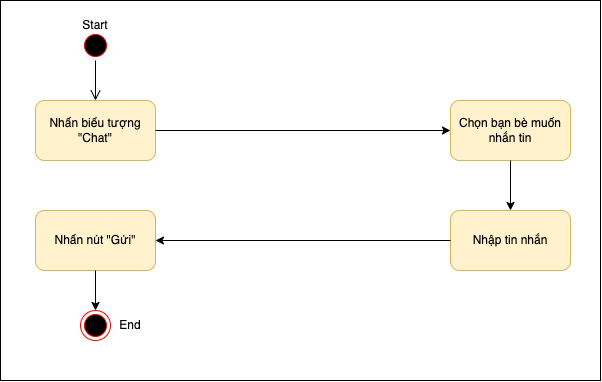
\includegraphics[width=12cm]{document/image/Chat.png}
  \captionof{figure}{Lược đồ Activity nhắn tin}
\end{center}

\subsection{Chức năng chia sẻ kế hoạch với bạn bè}
Đặc tả usecase chia sẻ kế hoạch với bạn bè: 
\begin{table}[H]
    \centering
	\begin{tabular}{|p{5cm}|p{10cm}|}
    
    \hline
    Usecase Name&Share kế hoạch với bạn bè\\
    \hline
    Usecase Description&Người dùng muốn share kế hoạch của mình với bạn bè\\
    \hline
    Post Condition&Hiển thị thông báo share thành công \\
    \hline
    Basic Flow& 1. Người dùng vào trang các kế hoạch đã tạo.
    
    2. Hiển thị danh sách các kế hoạch đã tạo.
    
    3. Nhấn vào biểu tượng "Share" trên bài.
    
    4. Hiển thị danh sách bạn bè.
    
    5. Nhấn chọn bạn bè muốn gởi.
    
    6. Nhấn "Share".
    
    5. Hiển thi thông báo thành công.\\
    

    \hline Business Rules& \\
   
   
	\hline
\end{tabular}
\caption{Usecase share kế hoạch}
\end{table}
 \begin{center}
  \captionsetup{type=figure}
  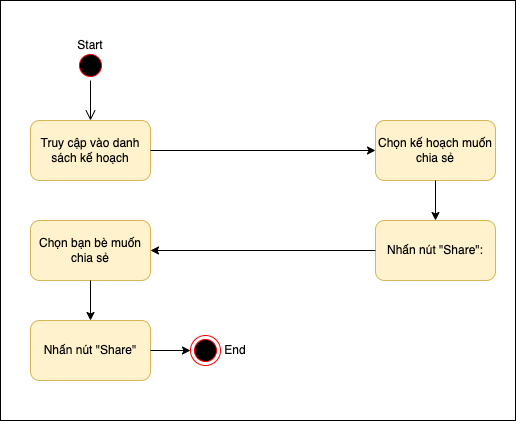
\includegraphics[width=12cm]{document/image/Share.png}
  \captionof{figure}{Lược đồ Activity share kế hoạch}
\end{center}
% \begin{figure}[H]
%     \centering
%     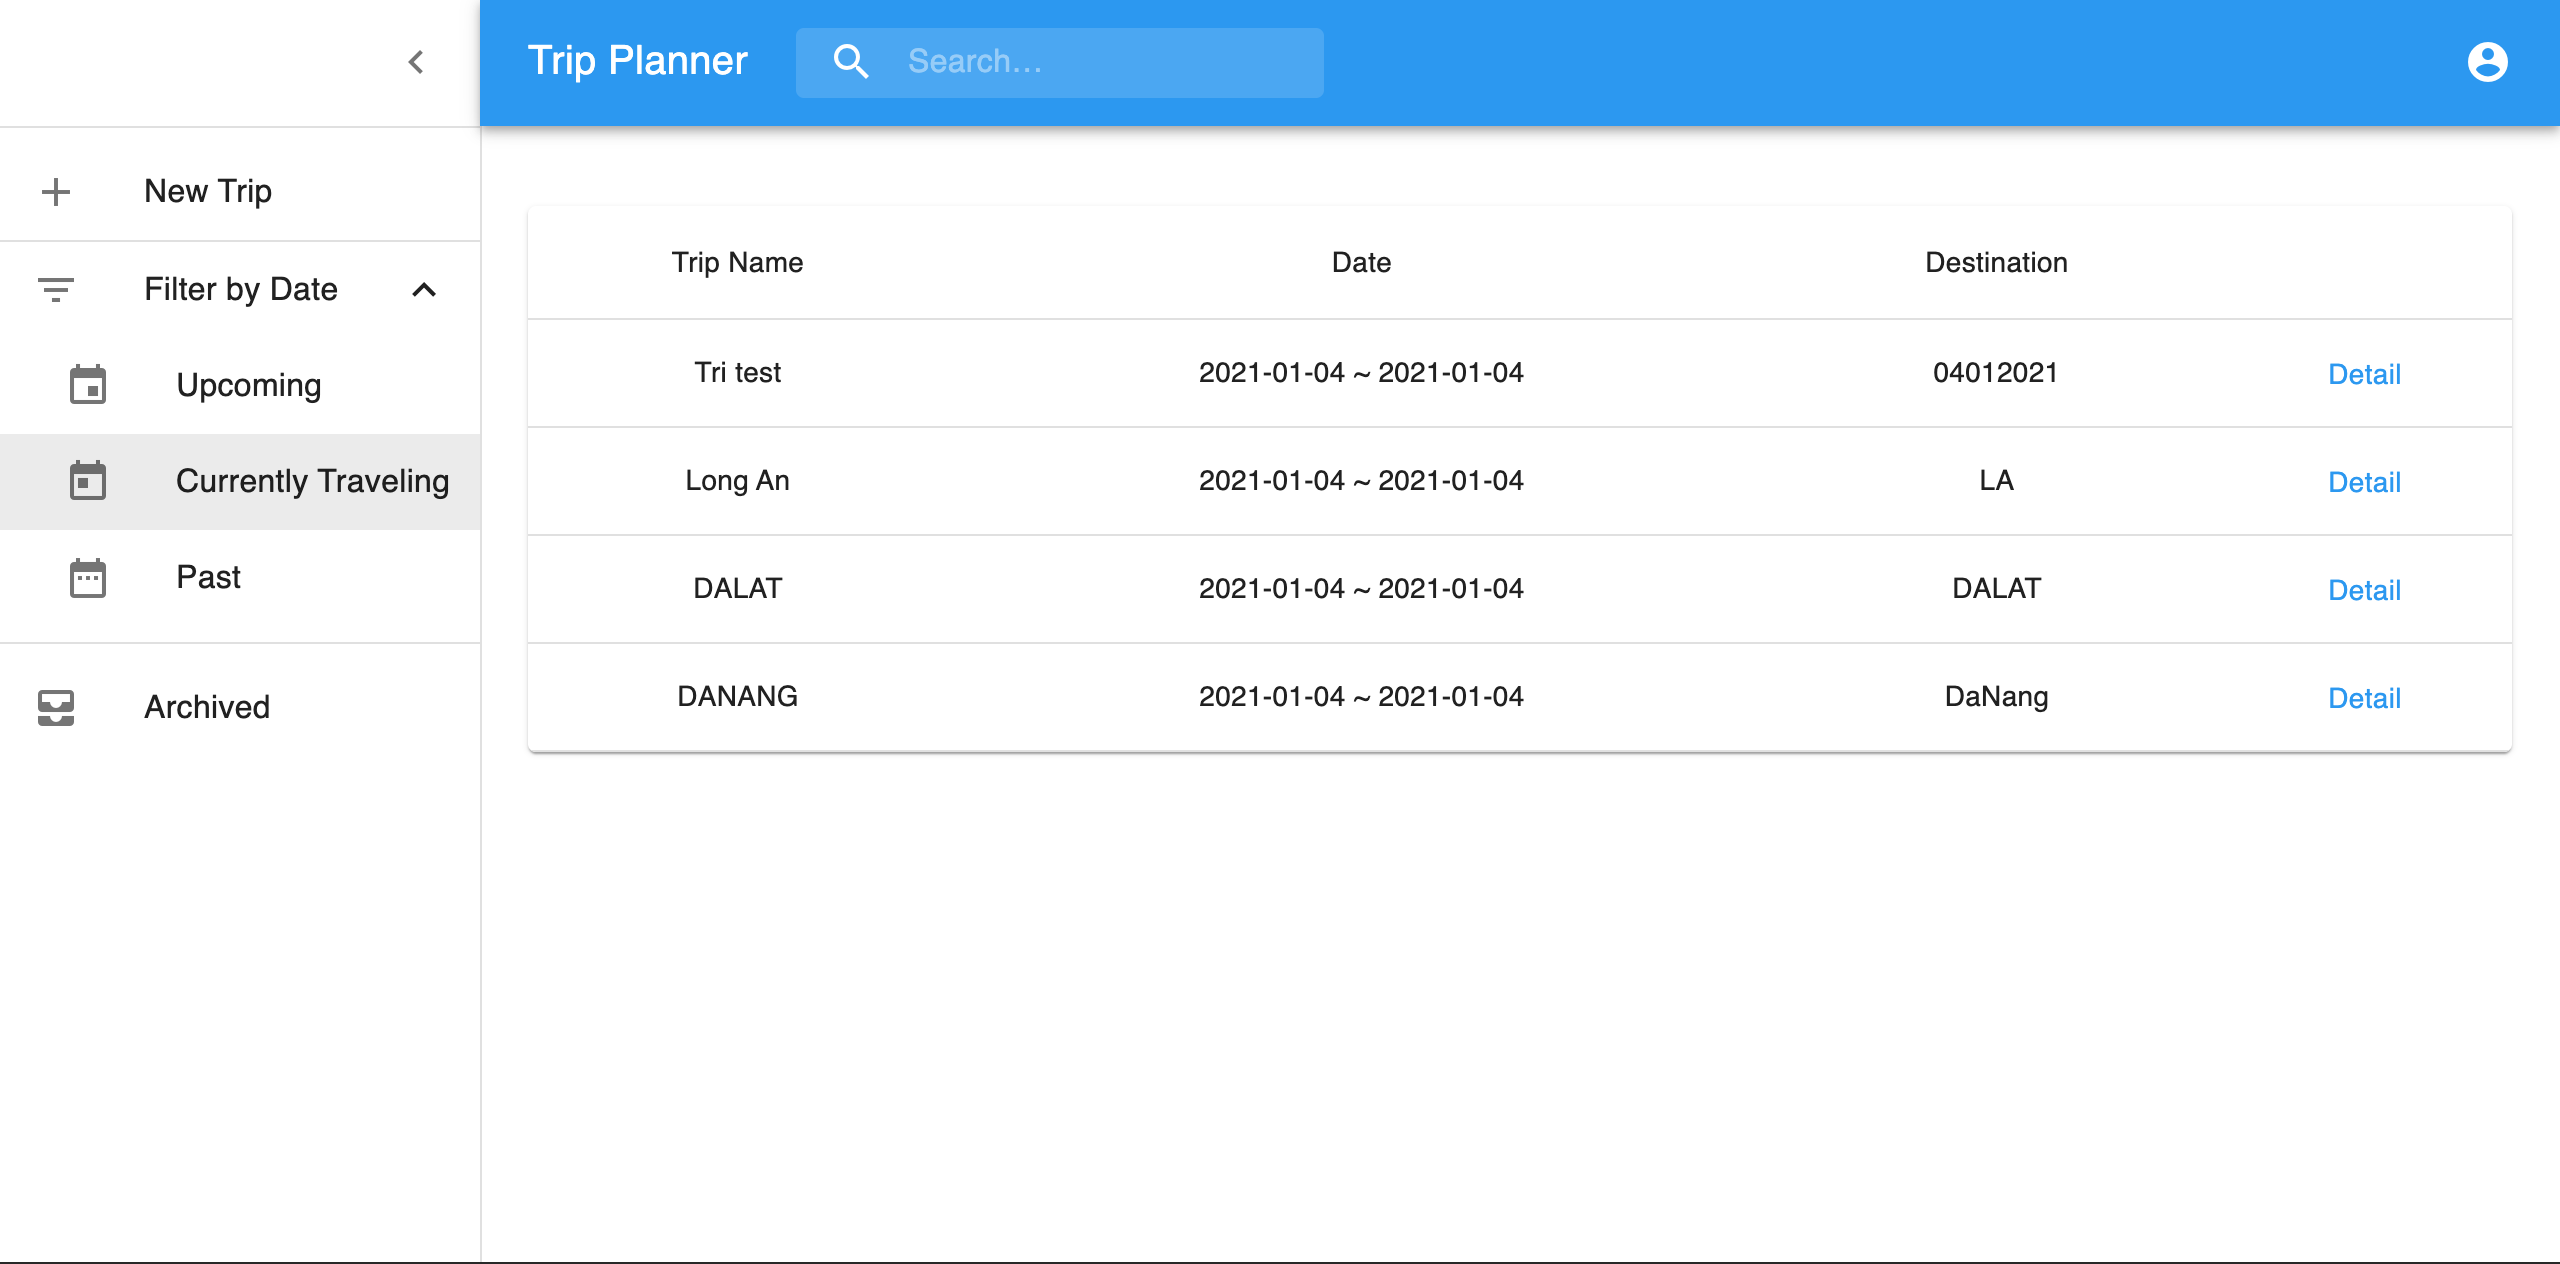
\includegraphics[width=15cm]{document/image/BangPlan.png}
%     \caption{Danh sách kế hoạch hiện có của người dùng}
%     \label{fig:fig_danh_sach_nguoi_dung}
% \end{figure}
 
% Danh sạch kế hoạch hiện có giúp người dùng có thể tự quản lý kế hoạch của mình cũng như các kế hoạch mình đã tham gia ( Past ). Người dùng có thể thêm xoá và sửa chữa thông tin trong kế hoạch của mình\\
% \begin{figure}[H]
%     \centering
%     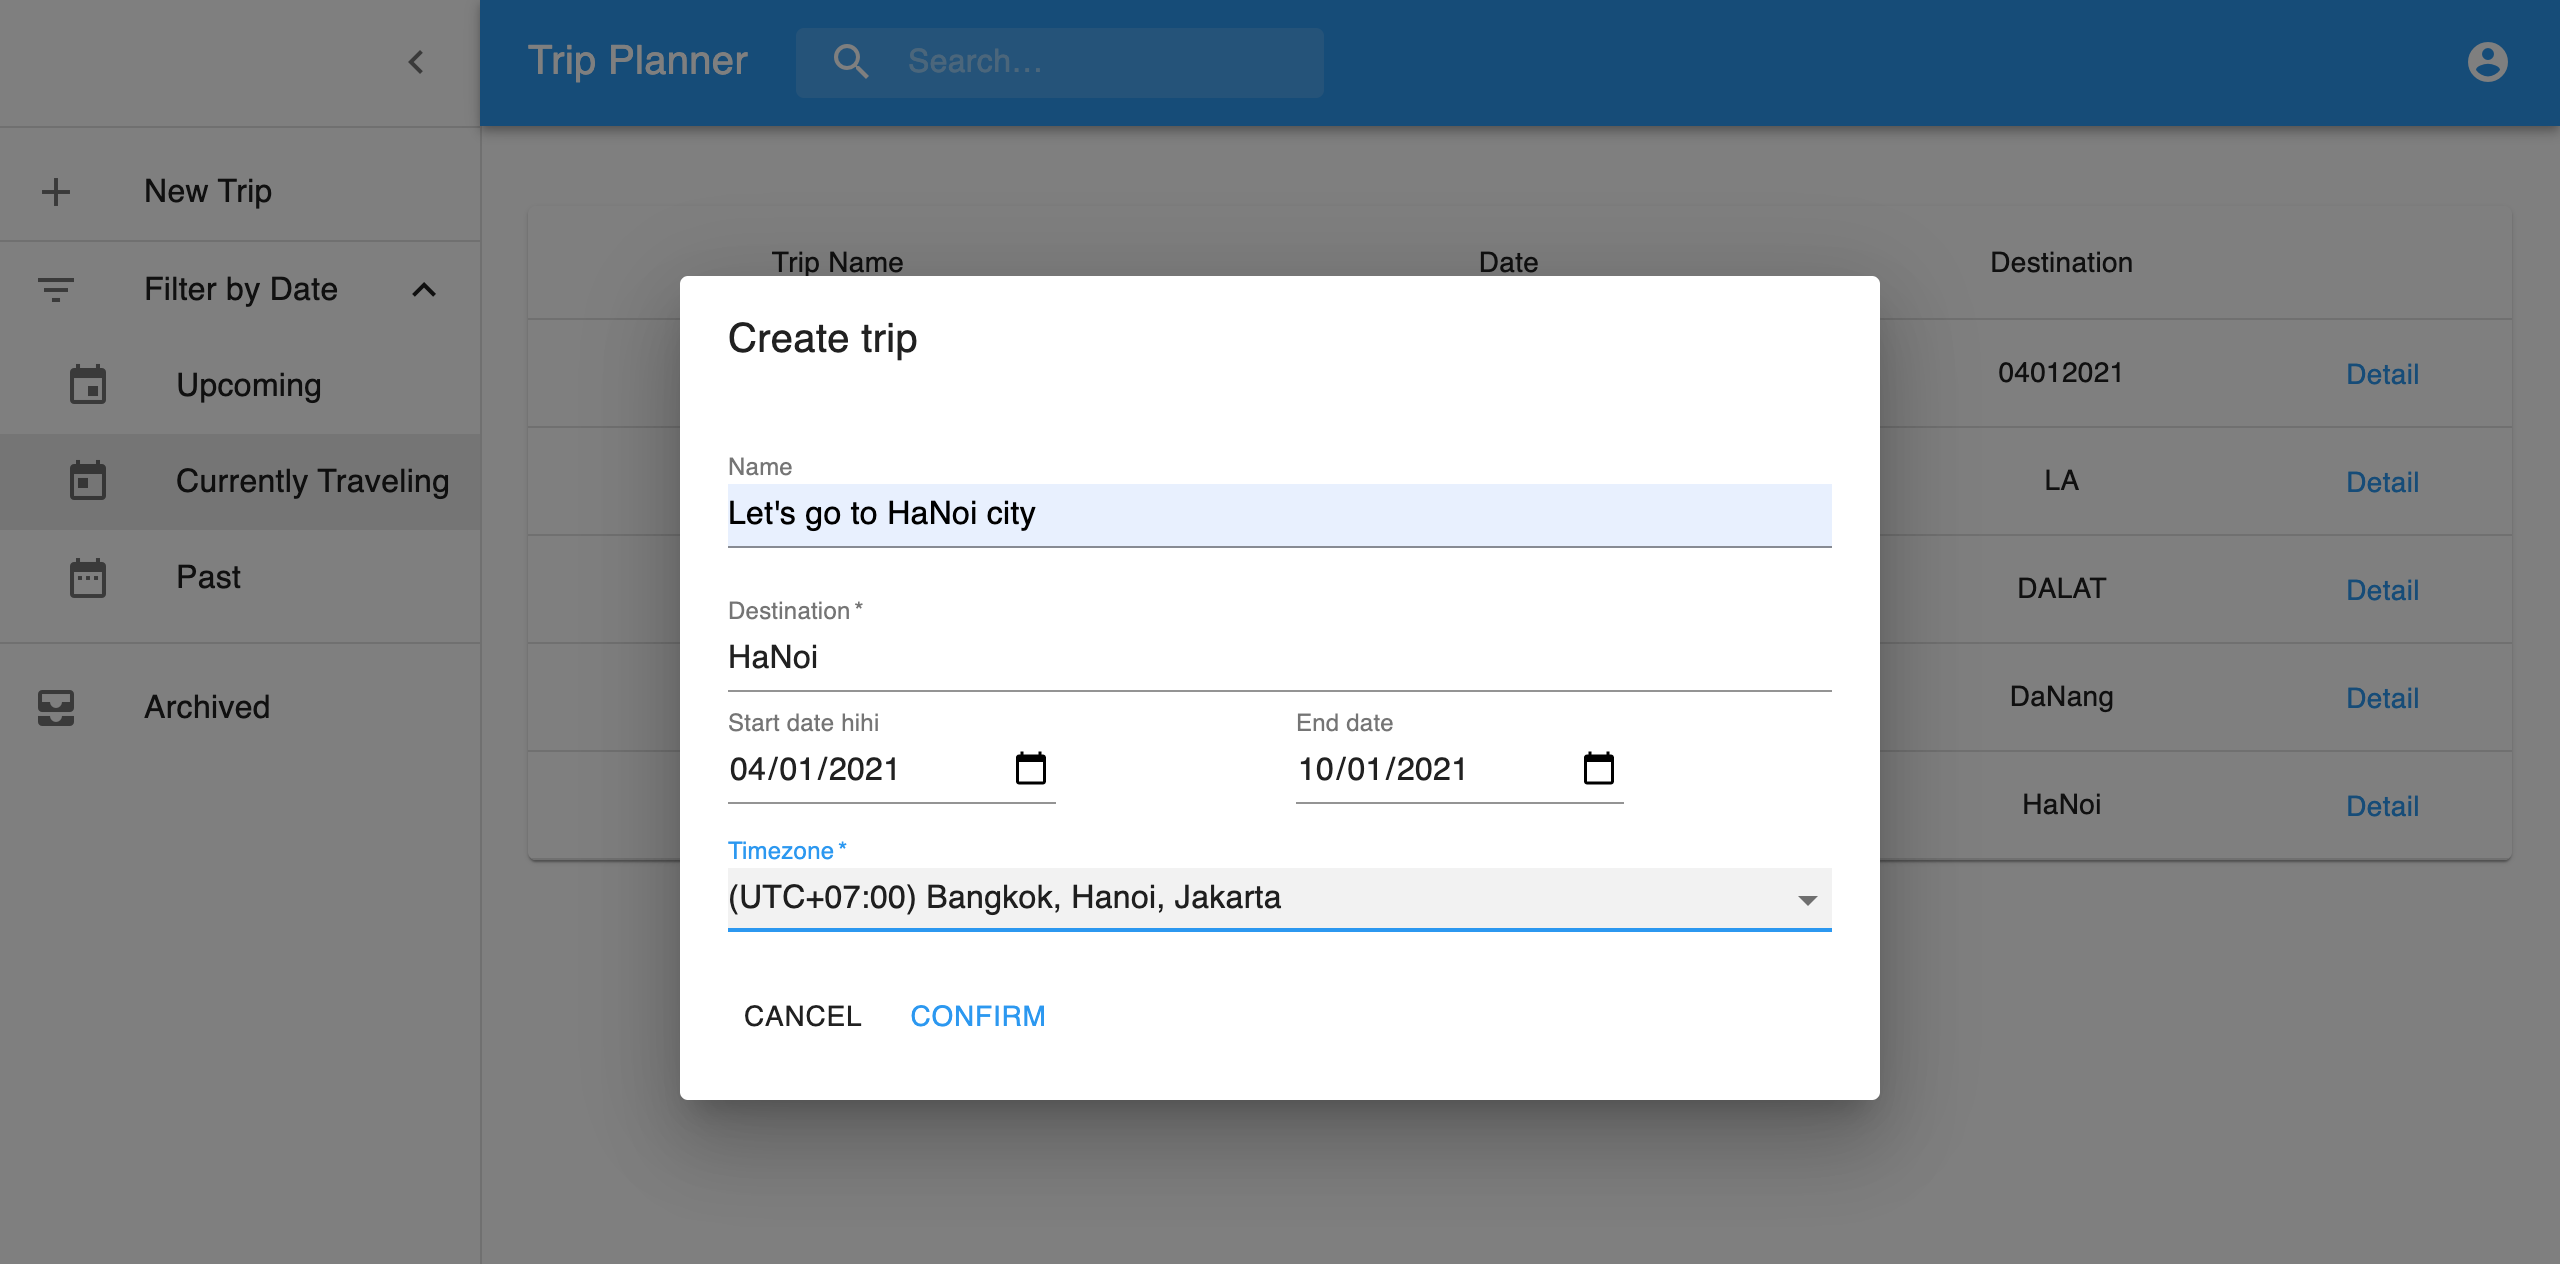
\includegraphics[width=15cm]{document/image/CreateNewPlan.png}
%     \caption{Thêm kế hoạch mới}
%     \label{fig:fig_edit_nguoi_dung}
% \end{figure}

% Khi đã tạo kế hoạch cho chuyến đi, người dùng có thể thêm các hoạt động chi tiết cho mỗi ngày đi \\

% \begin{figure}[H]
%     \centering
%     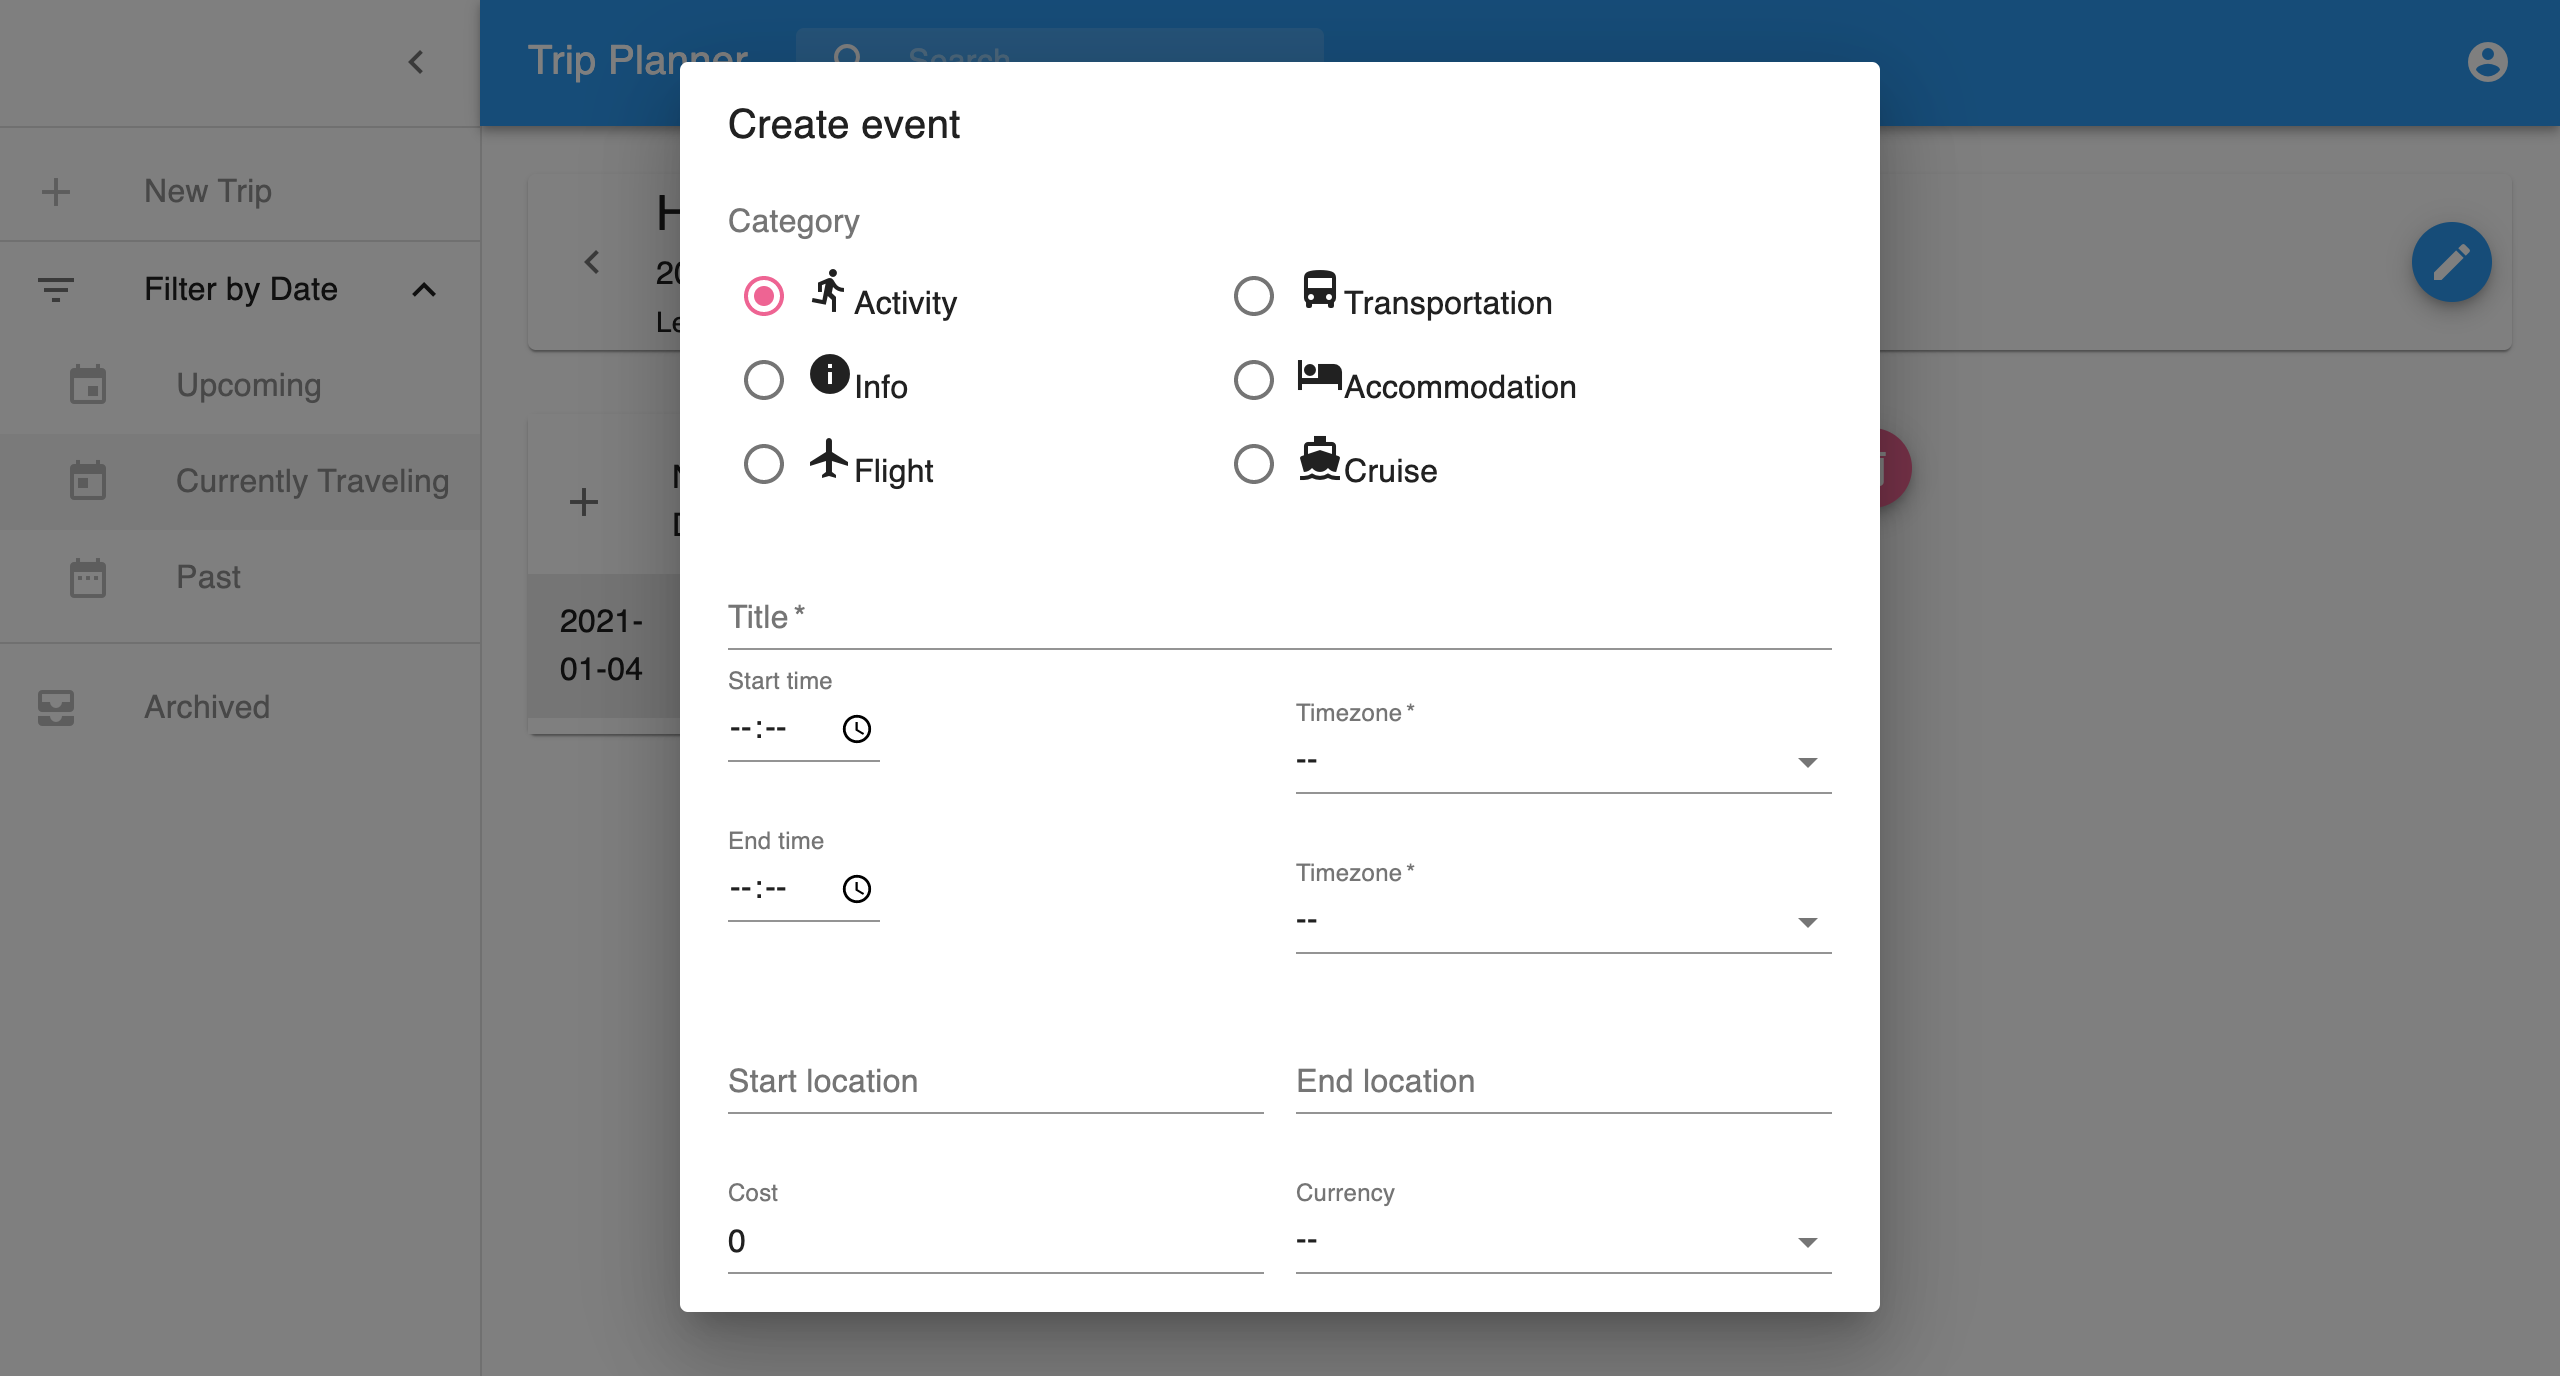
\includegraphics[width=15cm]{document/image/addActivity.png}
%     \caption{Thêm kế hoạch mới}
%     \label{fig:fig_edit_activity}
% \end{figure}

% Danh sách các hoạt động trong ngày giúp người dùng chủ động hơn về thời gian cho chuyến đi \\

% \begin{figure}[H]
%     \centering
%     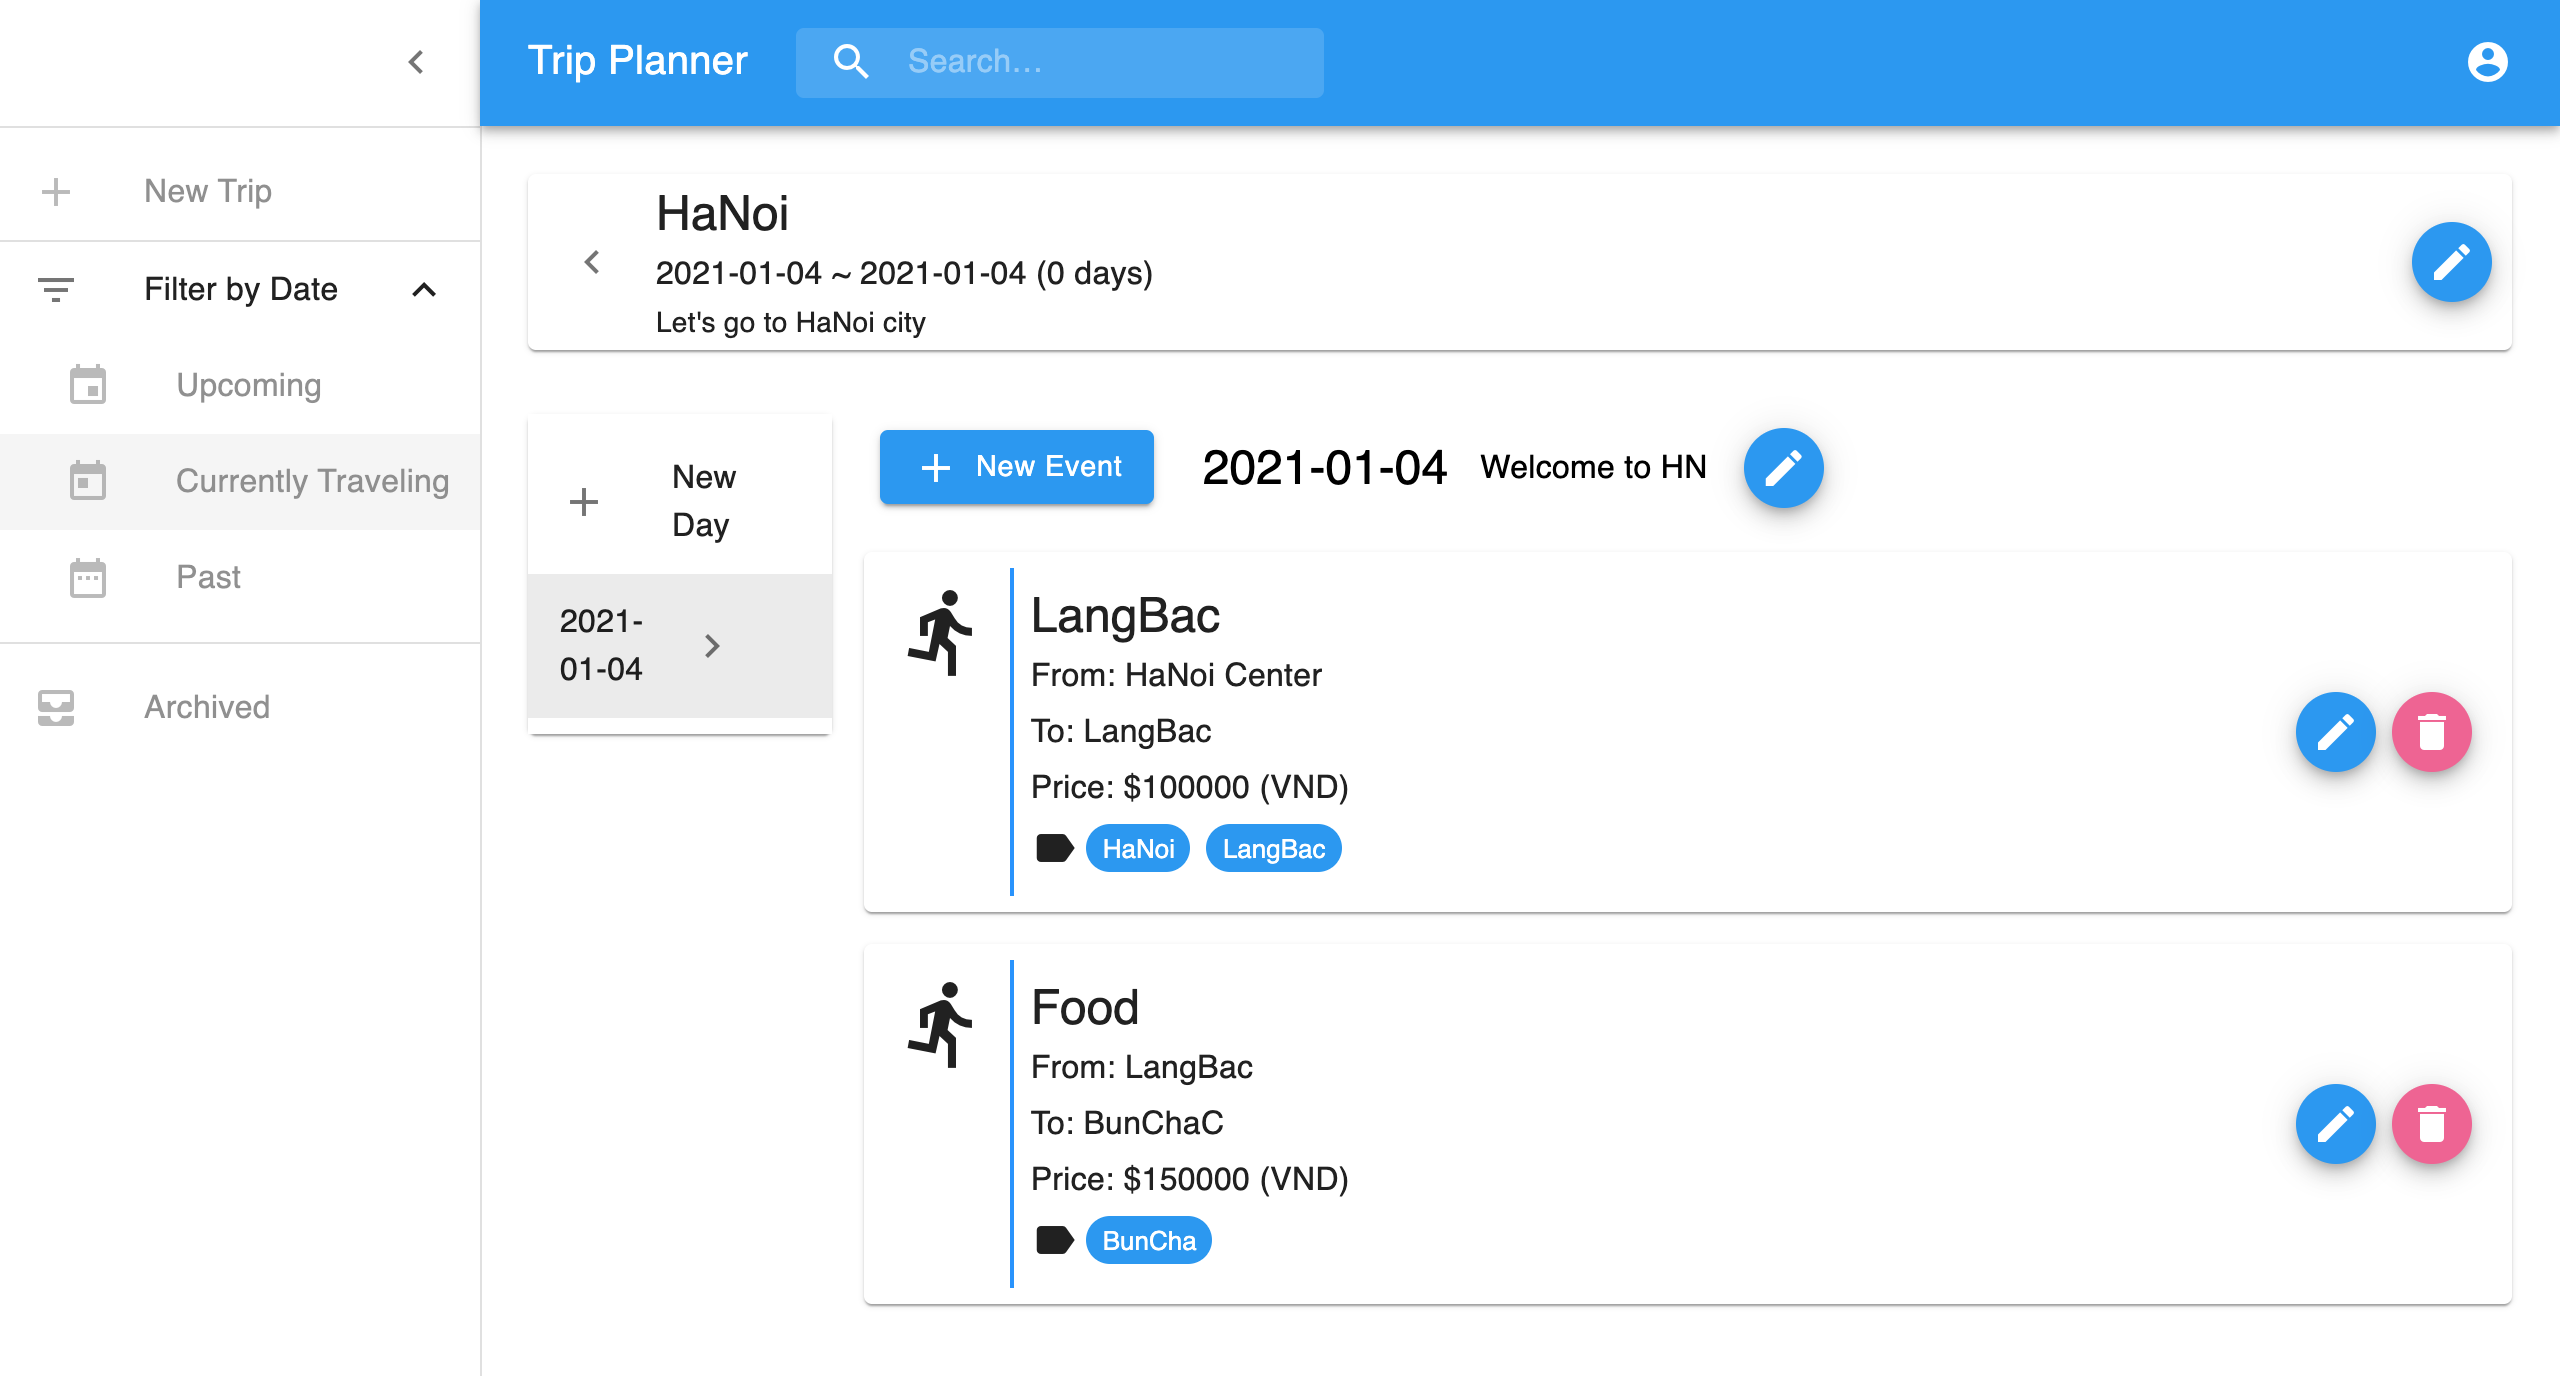
\includegraphics[width=15cm]{document/image/listActivity.png}
%     \caption{Danh sách hoạt động trong ngày}
%     \label{fig:fig_list_activity}
% \end{figure}


% \subsubsection{Chức năng: Quản lý}
% \begin{center}
%   \captionsetup{type=figure}
%   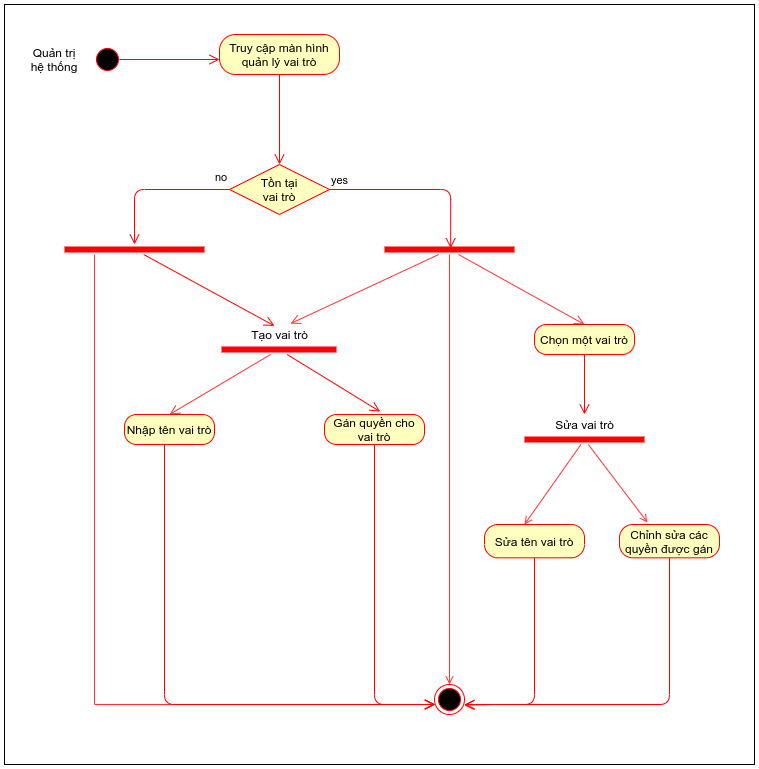
\includegraphics[width=15cm]{image/addRole.png}
%   \captionof{figure}{Lược đồ Activity quản lý vai trò hệ thống}
% \end{center}

% Hệ thống tồn tại cơ chế quản lý vai trò động. Mỗi vai trò được gán với các quyền truy cập. Quản trị viên có thể chỉnh sửa quyền của các vai trò một cách dễ dàng.\\
% \begin{center}
%   \captionsetup{type=figure}
%   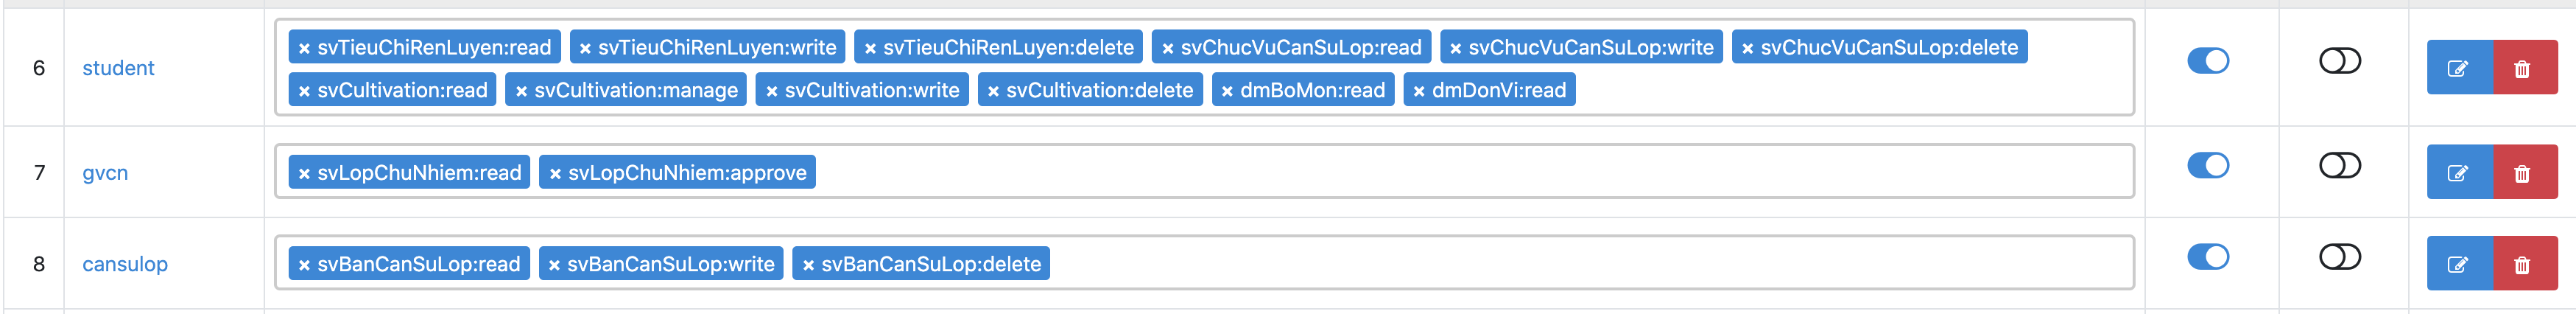
\includegraphics[width=15cm]{image/allrole.png}
%   \captionof{figure}{Danh sách vai trò có trong hệ thống hiện tại}
% \end{center}
% \subsection{Đối tượng: Cán bộ, công nhân viên của nhà trường}
% \subsubsection{Chức năng: Quản lý thông tin}
% \begin{center}
%   \captionsetup{type=figure}
%   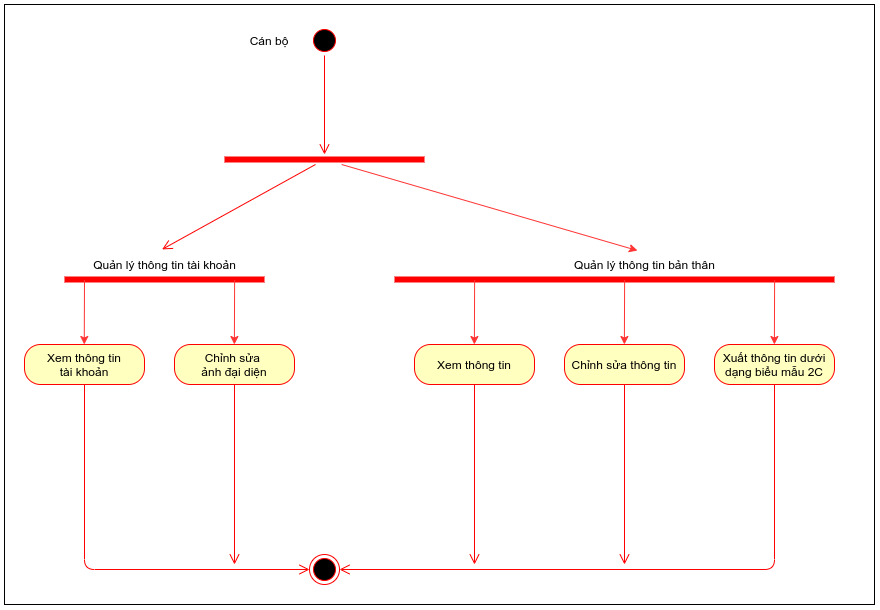
\includegraphics[width=15cm]{image/activityQLThongTin.png}
%   \captionof{figure}{Lược đồ Activity cho chức năng quản lý thông tin cho cán bộ}
% \end{center}

\section{Thiết kế UI Front-end hệ thống}

     Chính vì là hệ thống Website du lịch hỗ trợ người dùng tạo chi tiết chuyến đi nên Front-end là phần được nhóm em tập trung phát triển nhất.UI của hệ thống được nghiên cứu và thiết kế sao cho thân thiện và gây ấn tượng mạnh nhất với người dùng có thể.
     Về màu sắc và Logo cũng do nhóm tự thiết kế. Về UI của hệ thống đã được thiết kế như sau: 
     
     Chi tiết xem ở tài liệu đính kèm
     
     
% \subsection{Page Home}
% \begin{center}
%   \captionsetup{type=figure}
%   \includegraphics[width=12cm]{document/image/Web 1920 – 1.png}
%   \captionof{figure}{UI trang chủ.}
% \end{center}
% \clearpage
% \subsection{Page đăng nhập}
% \begin{center}
% \captionsetup{type=figure}
%   \includegraphics[width=12cm]{document/image/Web 1920 – 2.png}
%   \captionof{figure}{UI Trang đăng nhập.}
% \end{center}

% \subsection{Page List Bài Review}
% \begin{center}
% \captionsetup{type=figure}
%   \includegraphics[width=12cm]{document/image/Web 1920 – 3.png}
%   \captionof{figure}{UI Trang list bài review.}
% \end{center}

% \subsection{Page Bài Review}
% \begin{center}
% \captionsetup{type=figure}
%   \includegraphics[width=12cm]{document/image/Web 1920 – 4.png}
%   \captionof{figure}{UI bài review.}
% \end{center}


% \subsection{Page List Plan}
% \begin{center}
% \captionsetup{type=figure}
%   \includegraphics[width=12cm]{document/image/Web 1920 – 6.png}
%   \captionof{figure}{UI list Plan.}
% \end{center}
% \begin{center}
%   \captionsetup{type=figure}
%   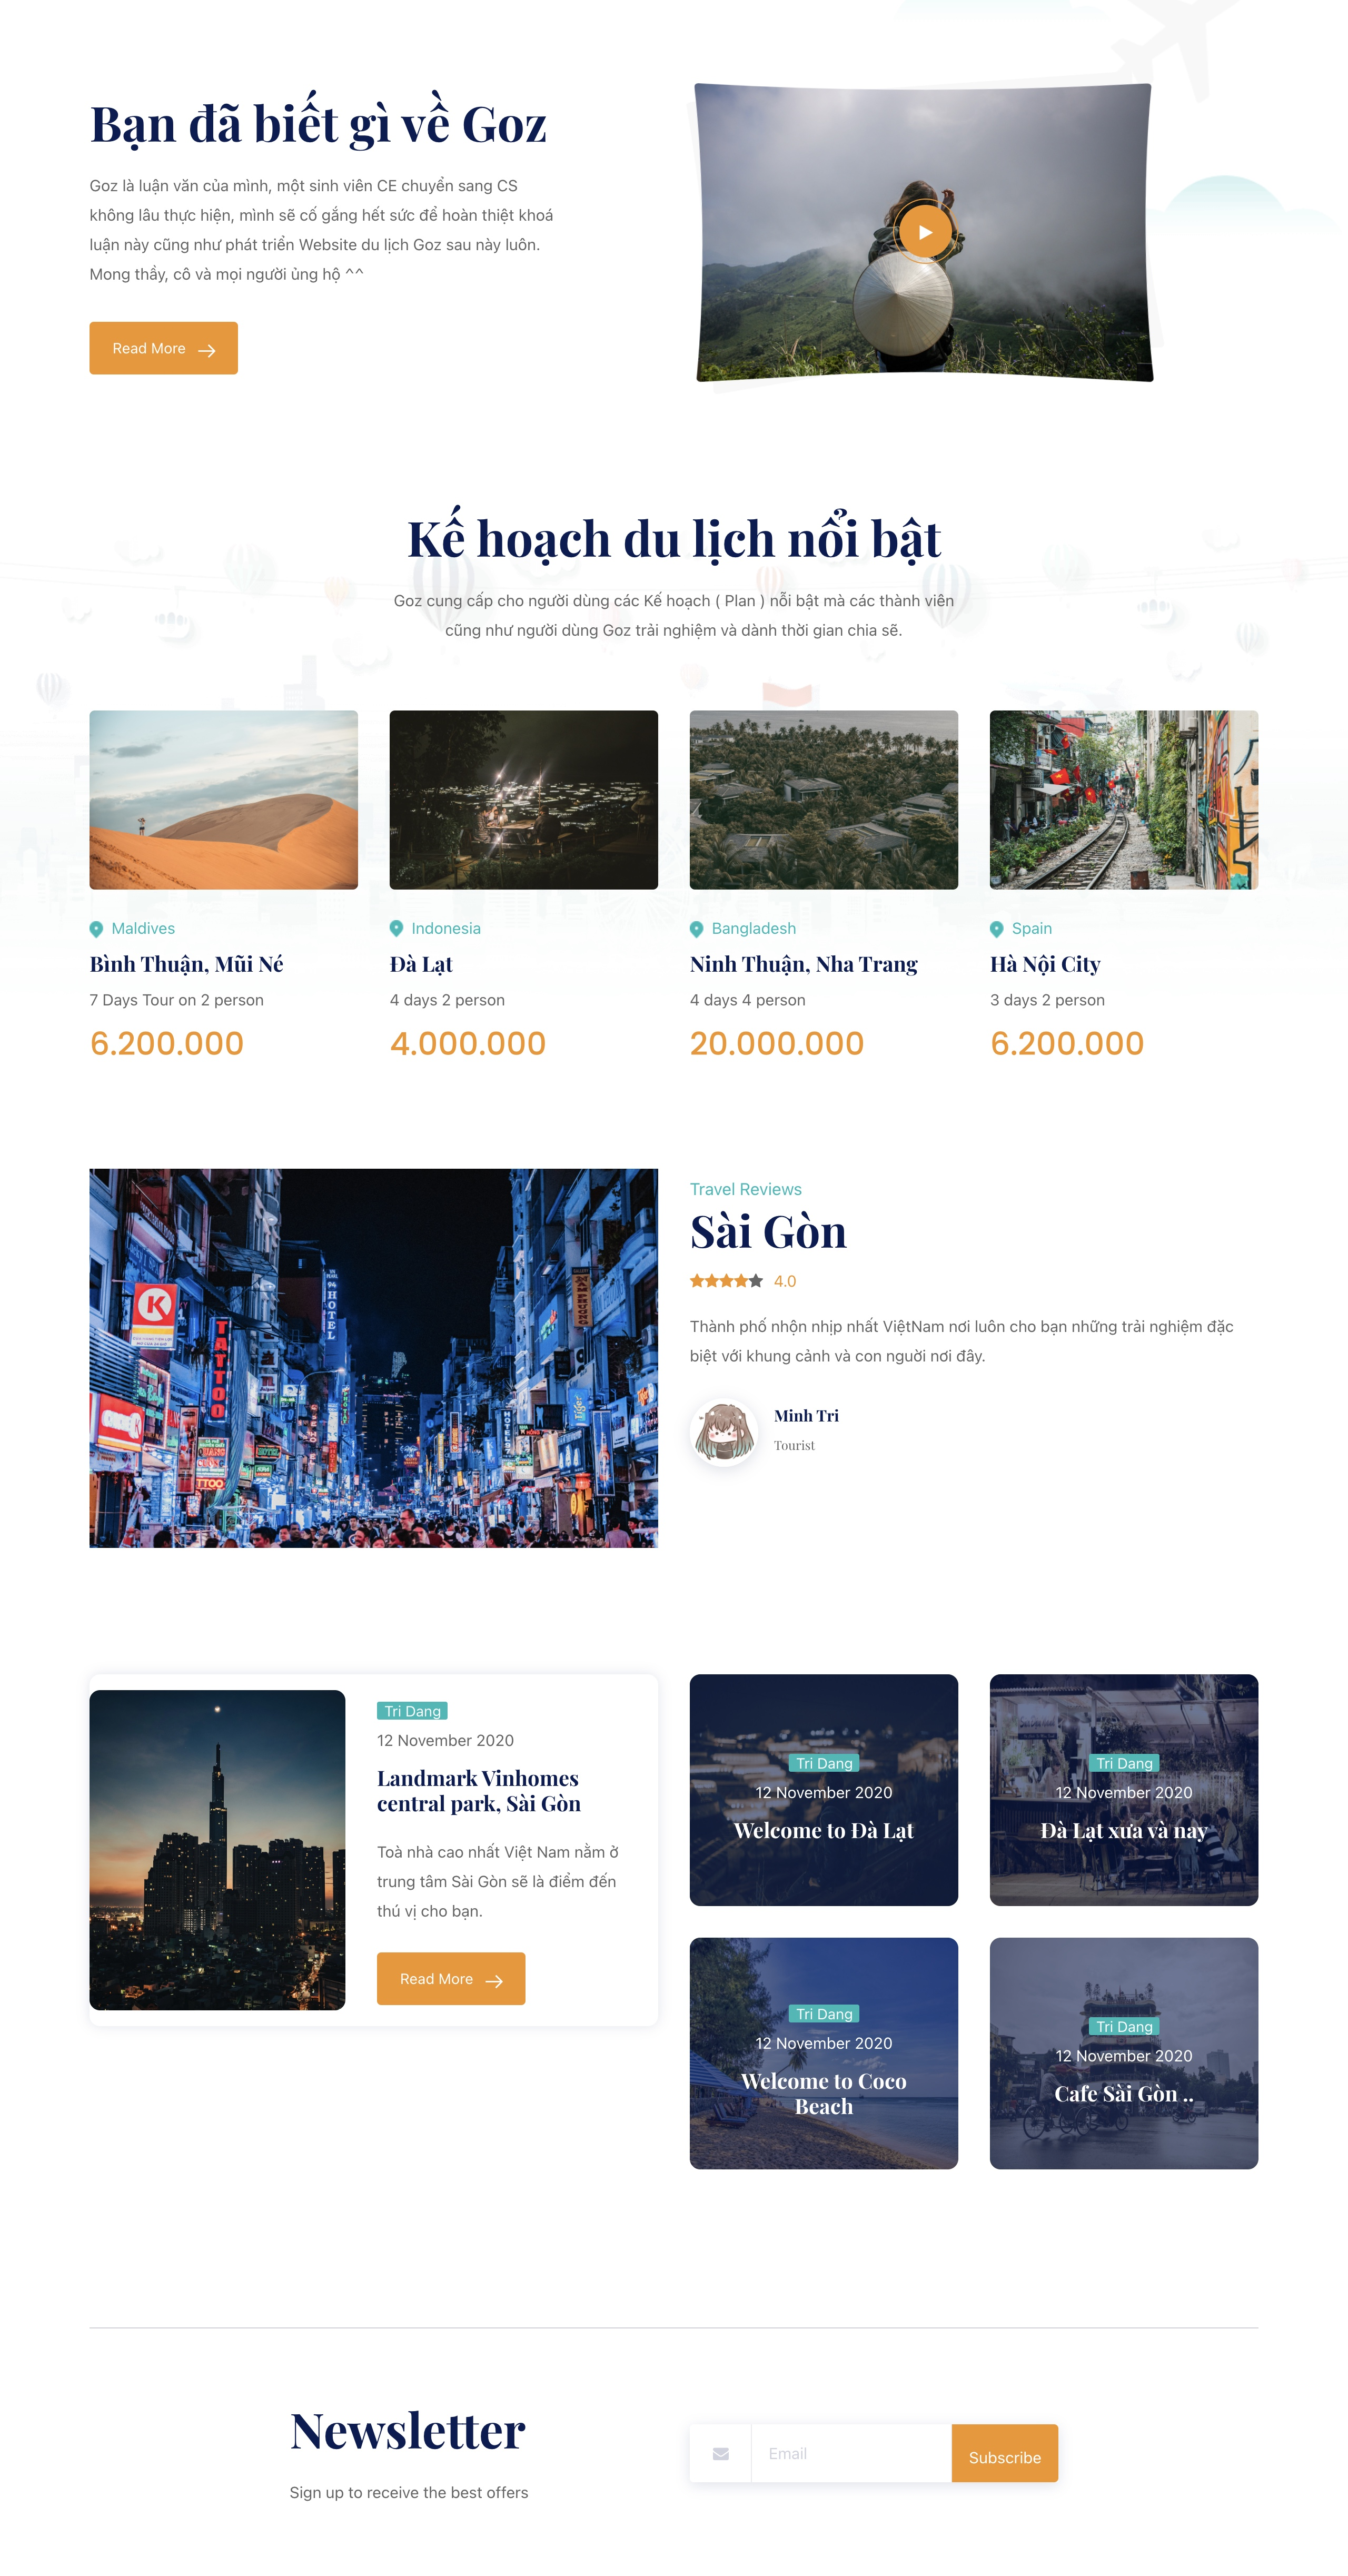
\includegraphics[width=12cm]{document/image/Home4.png}
%   \captionof{figure}{UI trang chủ.}
% \end{center}




